%%%%%%%%%%%%%%%%%%%%%%%%%%%%%%%%%%%%%%%%%%%%%%%%%%%%%%%%%%%%%%%%%%%%%
%% This is a (brief) model paper using the achemso class
%% The document class accepts keyval options, which should include
%% the target journal and optionally the manuscript type. 
%%%%%%%%%%%%%%%%%%%%%%%%%%%%%%%%%%%%%%%%%%%%%%%%%%%%%%%%%%%%%%%%%%%%%
\documentclass[journal=jacsat,manuscript=article]{achemso}
\SectionNumbersOn
\SubsectionNumbersOn
%\documentclass[12pt]{article}
%\usepackage[letterpaper,left=0.5in,right=0.5in,top=1.0in,bottom=1.0in]{geometry}

%%%%%%%%%%%%%%%%%%%%%%%%%%%%%%%%%%%%%%%%%%%%%%%%%%%%%%%%%%%%%%%%%%%%%
%% Place any additional packages needed here.  Only include packages
%% which are essential, to avoid problems later. Do NOT use any
%% packages which require e-TeX (for example etoolbox): the e-TeX
%% extensions are not currently available on the ACS conversion
%% servers.
%%%%%%%%%%%%%%%%%%%%%%%%%%%%%%%%%%%%%%%%%%%%%%%%%%%%%%%%%%%%%%%%%%%%%
\usepackage[version=3]{mhchem} % Formula subscripts using \ce{}
\usepackage{siunitx} % generating degrees Celsius in the document 
\usepackage{color}
\usepackage{soul} % allows highlighting text 
\usepackage{makecell}
\usepackage{booktabs}
\usepackage{amsmath}
\usepackage{amssymb}
\usepackage{gensymb}
\usepackage{verbatim}

\usepackage[utf8]{inputenc}
\usepackage{enumitem}
\usepackage{dsfont}
\usepackage{ulem}
\usepackage{hyperref}
\hypersetup{
    colorlinks=true,
    linkcolor=black,
    urlcolor=blue, 
    breaklinks=true,
    citecolor = red,
}
\usepackage{breakcites}
%\usepackage{caption}
\usepackage{float}
\usepackage[hang]{subfigure}
\usepackage{overpic}
\usepackage{listings}
\usepackage[super]{nth}
\usepackage{multicol}
\linespread{1.15}

%%%%%%%%%%%%%%%%%%%%%%%%%%%%%%%%%%%%%%%%%%%%%%%%%%%%%%%%%%%%%%%%%%%%%
%% If issues arise when submitting your manuscript, you may want to
%% un-comment the next line.  This provides information on the
%% version of every file you have used.
%%%%%%%%%%%%%%%%%%%%%%%%%%%%%%%%%%%%%%%%%%%%%%%%%%%%%%%%%%%%%%%%%%%%%
%%\listfiles

%%%%%%%%%%%%%%%%%%%%%%%%%%%%%%%%%%%%%%%%%%%%%%%%%%%%%%%%%%%%%%%%%%%%%
%% Place any additional macros here.  Please use \newcommand* where
%% possible, and avoid layout-changing macros (which are not used
%% when typesetting).
%%%%%%%%%%%%%%%%%%%%%%%%%%%%%%%%%%%%%%%%%%%%%%%%%%%%%%%%%%%%%%%%%%%%%
\newcommand*\mycommand[1]{\texttt{\emph{#1}}}
\DeclareRobustCommand
  \Compactcdots{\mathinner{\cdotp\mkern-2mu\cdotp\mkern-2mu\cdotp}}

%%%%%%%%%%%%%%%%%%%%%%%%%%%%%%%%%%%%%%%%%%%%%%%%%%%%%%%%%%%%%%%%%%%%%
%% Meta-data block
%% ---------------
%% Each author should be given as a separate \author command.
%%
%% Corresponding authors should have an e-mail given after the author
%% name as an \email command. Phone and fax numbers can be given
%% using \phone and \fax, respectively; this information is optional.
%%
%% The affiliation of authors is given after the authors; each
%% \affiliation command applies to all preceding authors not already
%% assigned an affiliation.
%%
%% The affiliation takes an option argument for the short name.  This
%% will typically be something like "University of Somewhere".
%%
%% The \altaffiliation macro should be used for new address, etc.
%% On the other hand, \alsoaffiliation is used on a per author basis
%% when authors are associated with multiple institutions.
%%%%%%%%%%%%%%%%%%%%%%%%%%%%%%%%%%%%%%%%%%%%%%%%%%%%%%%%%%%%%%%%%%%%%
\author{Stephen P. Vicchio}
\affiliation[Clemson University]
{Department of Chemical and Biomolecular Engineering, Clemson University, Clemson, SC}
\author{Zhihengyu Chen}
\affiliation[Stony Brook University]
{Department of Chemistry, Stony Brook University, Stony Brook, NY}
\author{Karena Chapman}
\affiliation[Stony Brook University]
{Department of Chemistry, Stony Brook University, Stony Brook, NY}
\author{Rachel B. Getman}
\email{rgetman@g.clemson.edu}
\affiliation[Clemson University]
{Department of Chemical and Biomolecular Engineering, Clemson University, Clemson, SC}

%%%%%%%%%%%%%%%%%%%%%%%%%%%%%%%%%%%%%%%%%%%%%%%%%%%%%%%%%%%%%%%%%%%%%
%% The document title should be given as usual. Some journals require
%% a running title from the author: this should be supplied as an
%% optional argument to \title.
%%%%%%%%%%%%%%%%%%%%%%%%%%%%%%%%%%%%%%%%%%%%%%%%%%%%%%%%%%%%%%%%%%%%%
\title[manuscript]{
Supporting Information:\\Identifying the structure and composition of \ce{Ni(II)}-hydroxo catalyst supported the NU-1000 metal-organic framework
}

%%%%%%%%%%%%%%%%%%%%%%%%%%%%%%%%%%%%%%%%%%%%%%%%%%%%%%%%%%%%%%%%%%%%%
%% Some journals require a list of abbreviations or keywords to be
%% supplied. These should be set up here, and will be printed after
%% the title and author information, if needed.
%%%%%%%%%%%%%%%%%%%%%%%%%%%%%%%%%%%%%%%%%%%%%%%%%%%%%%%%%%%%%%%%%%%%%
\abbreviations{IR,NMR,UV}
\keywords{American Chemical Society, \LaTeX}

%%%%%%%%%%%%%%%%%%%%%%%%%%%%%%%%%%%%%%%%%%%%%%%%%%%%%%%%%%%%%%%%%%%%%
%% The manuscript does not need to include \maketitle, which is
%% executed automatically.
%%%%%%%%%%%%%%%%%%%%%%%%%%%%%%%%%%%%%%%%%%%%%%%%%%%%%%%%%%%%%%%%%%%%%
\begin{document}
%%%%%%%%%%%%%%%%%%%%%%%%%%%%%%%%%%%%%%%%%%%%%%%%%%%%%%%%%%%%%%%%%%%%%
%% Start the table of content here
%%%%%%%%%%%%%%%%%%%%%%%%%%%%%%%%%%%%%%%%%%%%%%%%%%%%%%%%%%%%%%%%%%%%%

\newpage
\tableofcontents

%%%%%%%%%%%%%%%%%%%%%%%%%%%%%%%%%%%%%%%%%%%%%%%%%%%%%%%%%%%%%%%%%%%%%
%% Start the main part of the manuscript here.
%%%%%%%%%%%%%%%%%%%%%%%%%%%%%%%%%%%%%%%%%%%%%%%%%%%%%%%%%%%%%%%%%%%%%

\newpage
\section{Computational Methodology}

\subsection{Schematic for \textit{ab initio} thermodynamic analysis}
    \begin{figure}[H]
        \centering
        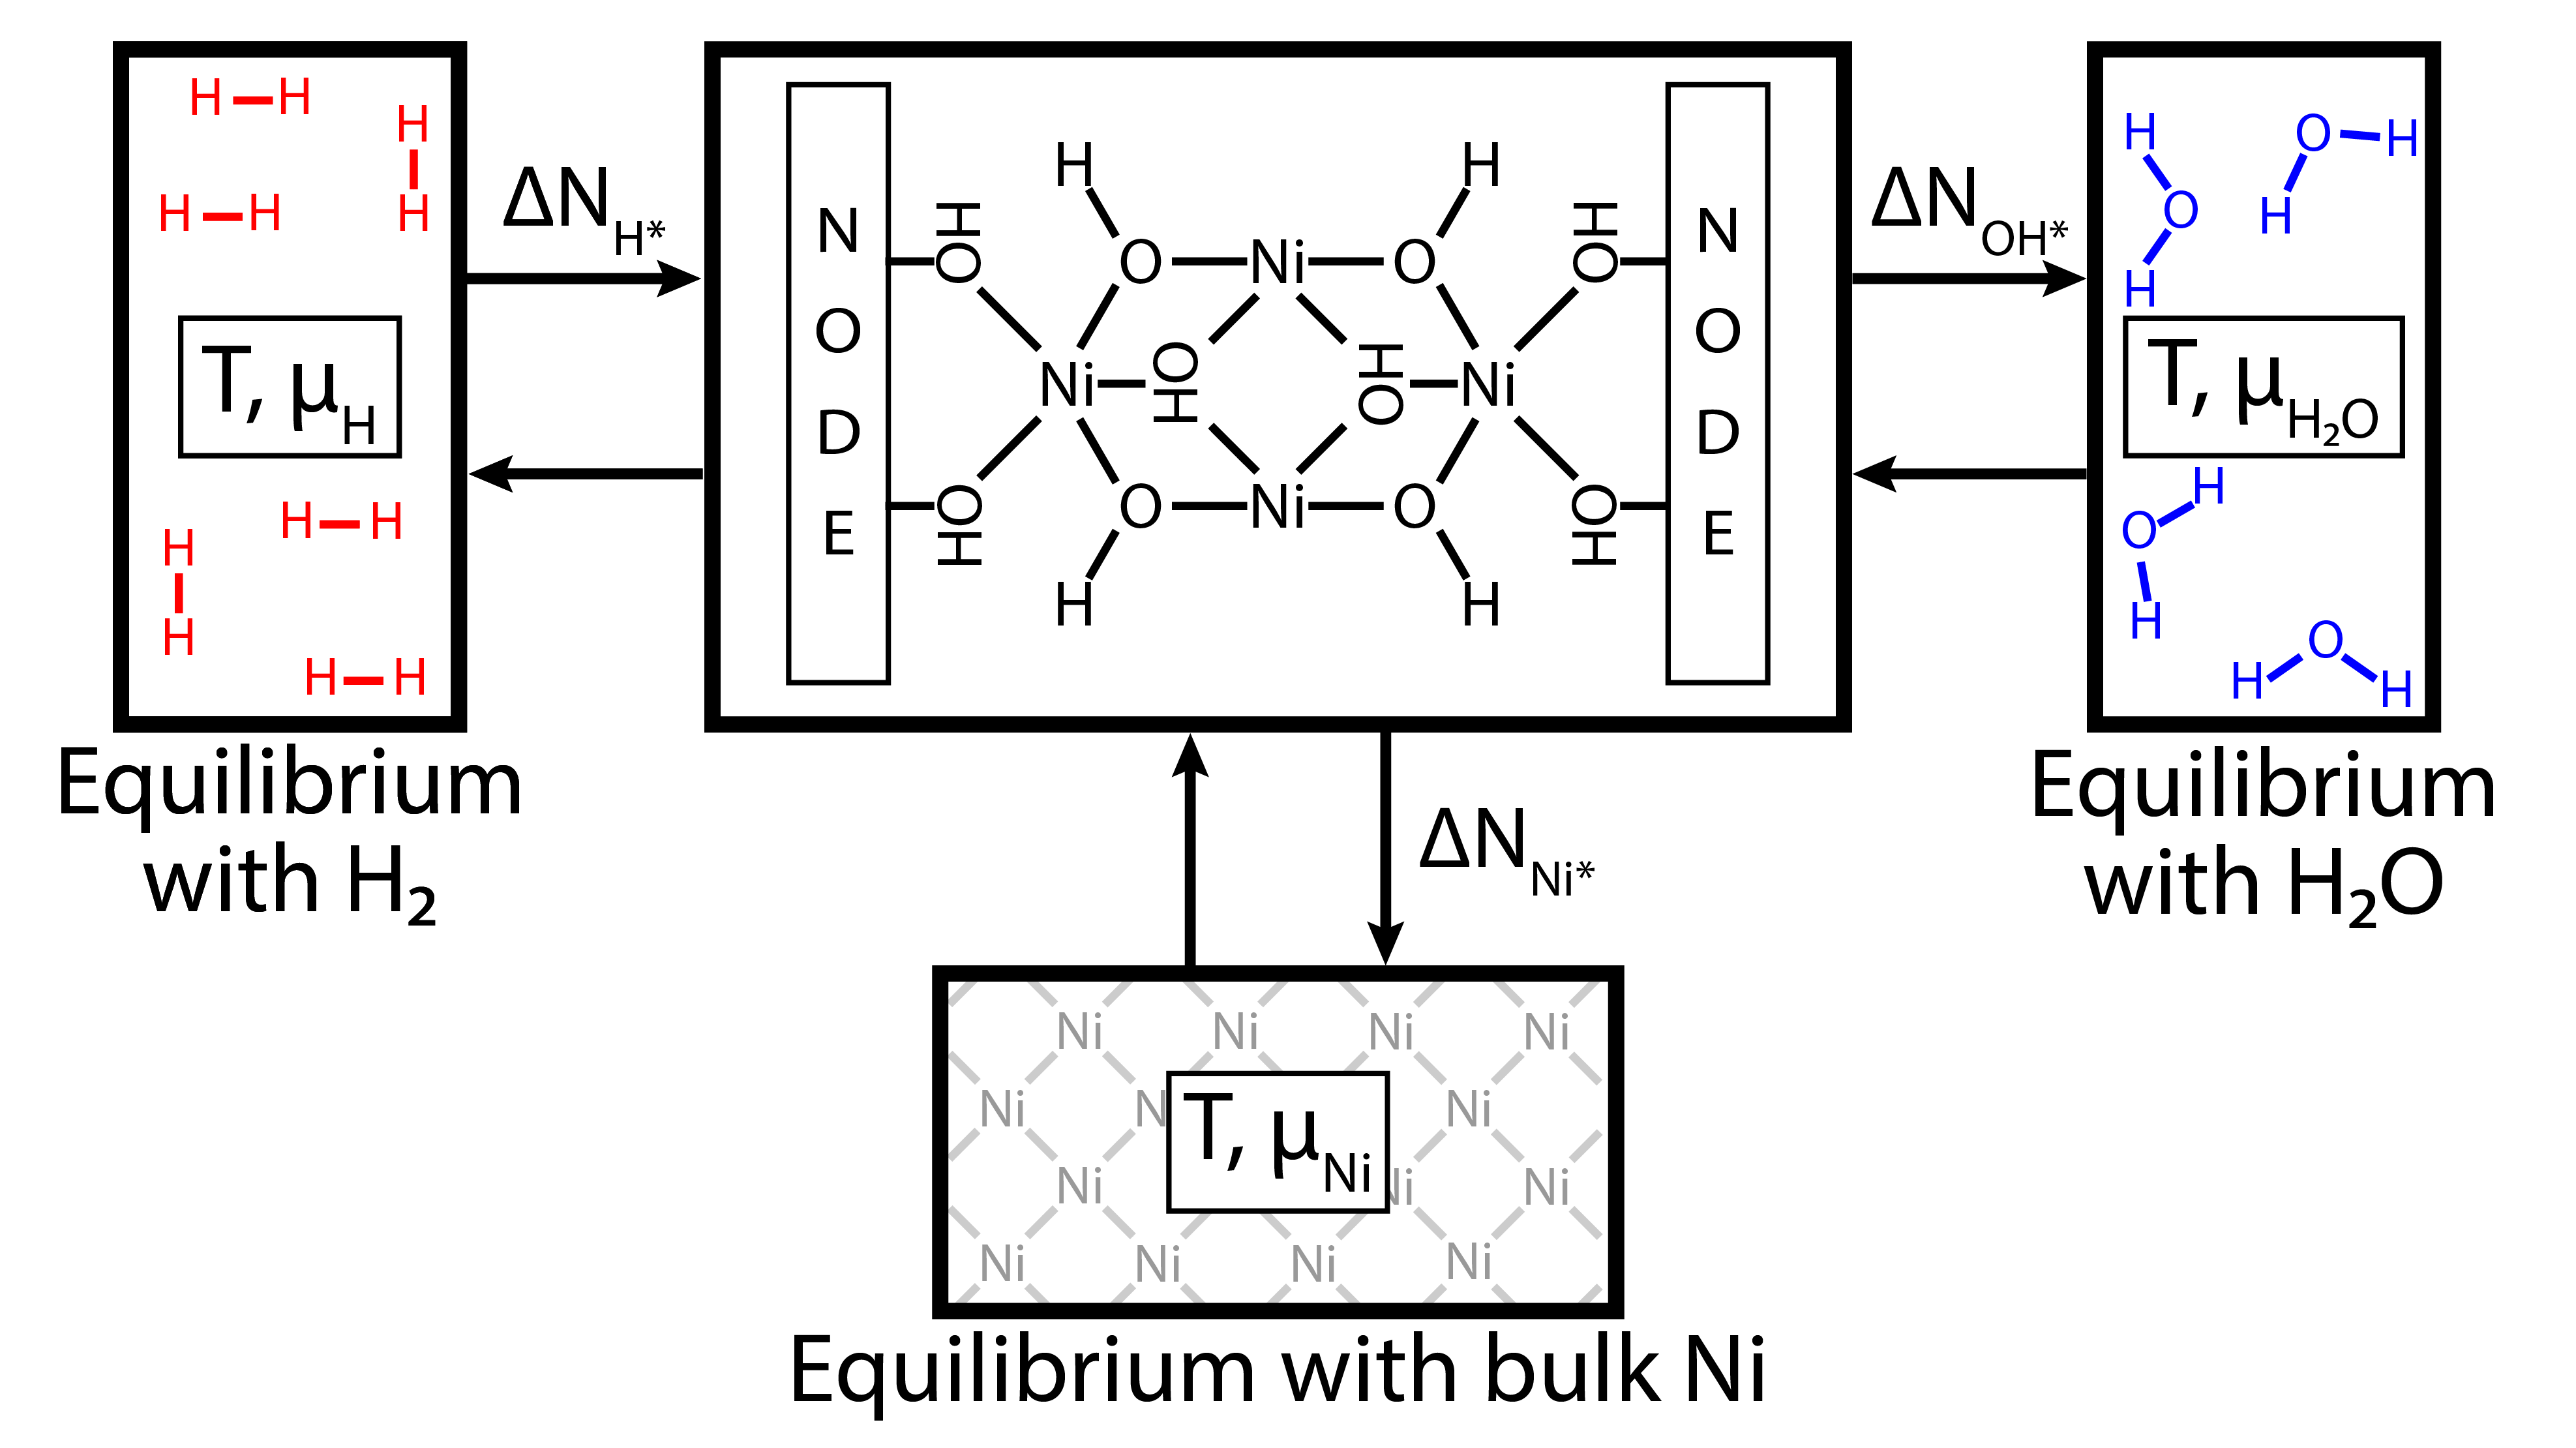
\includegraphics{zi-images/00-General-Graphics/FPT-schematic-full.png}
        \caption{Diagram showing the assumed equilibria necessary to transform with \ce{\text{H}^{*}}, \ce{\text{OH}^{*}}, \ce{Ni^{*}} for the \textit{ab initio} thermodynamic analysis method. The assume assumed equilibria capture the reaction conditions influences on the stability of the metal cluster.}
        \label{fig:SI-FPT-process-diagram}
    \end{figure}

    Figure \ref{fig:SI-FPT-process-diagram} shows the \textit{ab initio} thermodynamic analysis process we used to evaluate the stability of a \ce{Ni4}-cluster supported on the NU-1000 MOF. We assume the cluster is in equilibrium with three different reservoirs, which allows for transformations with respect to \ce{H^{*}}, \ce{OH^{*}}, and \ce{Ni^{*}}. We derive expressions relating the chemical potentials for each transformed species to their respective bulk reservoirs.   

    \newpage
    
    
\subsection{Deriving the free energy expressions}
We transform the free energy from a fixed number of atoms to a fixed chemical potential to account for the compositional variation of the different activated clusters (Equation \ref{eq:transformation1}):
\begin{equation}
    F^{0}(T,P,N_{\text{H}^{*}},N_{\text{OH}^{*}},N_{\text{Ni}^{*}}) \rightarrow F^{3}(T,P,\mu_{\text{H}^{*}},\mu_{\text{OH}^{*}},\mu_{\text{Ni}^{*}})
    \label{eq:transformation1}
\end{equation}
where $N_{\text{H}^{*}}$ is the number of adsorbed \ce{H} on the cluster with chemical potential $\mu_{\text{H}^{*}}$, $N_{\text{OH}^{*}}$ is the number of adsorbed \ce{OH} on the cluster with chemical potential $\mu_{\text{OH}^{*}}$, and $N_{\text{Ni}^{*}}$ is the number of adsorbed metal species (\ce{Ni}) on the cluster with chemical potential $\mu_{\text{Ni}^{*}}$. We write the transformed free energy expressions as Equation \ref{eq:transformation2}:
\begin{equation}
    \begin{split}
        F^{3}(T,P,\mu_{\text{H}^{*}},\mu_{\text{OH}^{*}},\mu_{\text{Ni}^{*}}) &= F^{0}(T,P,N_{\text{H}^{*}},N_{\text{OH}^{*}},N_{\text{Ni}^{*}}) \\ &- (\mu_{\text{H}^{*}})(N_{\text{H}^{*}}) \\ &- (\mu_{\text{OH}^{*}})(N_{\text{OH}^{*}}) \\ &- (\mu_{\text{Ni}^{*}})(N_{\text{Ni}^{*}})  
        \label{eq:transformation2}    
    \end{split}
\end{equation}
Equation \ref{eq:transformation2} allows  for compositionally different structures to be compared with the gas phase conditions being included in the free energy expression. The free energy between two different structures, defined modified ($k$) and reference ($i$), is determined by Equation \ref{eq:freenergyfinal}:
\begin{equation}
    \begin{split}
        \Delta F^{(3)}(T,\mu_{\text{H}^{*}},\mu_{\text{OH}^{*}},\mu_{\text{Ni}^{*}})  = 
        & F_{j}(T,N_{j,\text{H}^{*}},N_{j,\text{OH}^{*}},N_{j,\text{Ni}^{*}}) - 
          F_{i}(T,N_{i,\text{H}^{*}},N_{i,\text{OH}^{*}},N_{i,\text{Ni}^{*}}) \\
        & - (\mu_{\text{H}^{*}})(\Delta N_{\text{H}^{*}}) - (\mu_{\text{OH}^{*}})(\Delta N_{\text{OH}^{*}}) - (\mu_{\text{Ni}^{*}})(\Delta N_{\text{Ni}^{*}}) \\ 
    \end{split}
    \label{eq:freenergyfinal}
\end{equation}
where $\Delta N_{i}$ terms represent the different between the modified ($N_{j}$) and reference ($N_{i}$) structures for a particular species. The $^{*}$ indicates the species is bound to the cluster. The reference structure is the \ce{Ni4(OH)6.4H2O} cluster, which was initially proposed by \citeauthor{PlateroPrats2017} \cite{PlateroPrats2017} The model consists of \ce{OH}-ligands linking the \ce{Ni} atoms. Our goal is to determine the influence of reaction conditions on the thermodynamic stability of the \ce{Ni4}-cluster, which we accomplish by relating the free energy expression to the reaction conditions, temperature ($T$) and pressure ($P$) using the chemical potential terms. The assumed equilibrium (Figure \ref{fig:SI-FPT-process-diagram}) relate the chemical potential of the gas phase species to the chemical of the adsorbed species. The following sections derive the necessary equilibrium expression. 

\subsubsection{Equilibrium expression for $\text{H}^{*}$}
For $H^{*}$, the assumed equilibrium is with a reservoir of \ce{H2} gas:
\begin{equation}
    \frac{1}{2} H_{2} \ce{<=>} H^{*}
\end{equation}
where the chemical potential terms are related by: 
\begin{equation}
    \frac{1}{2} \mu_{H_{2}}^{g}(T,P) = \mu_{\text{H}^{*}}
\end{equation}  
The $\mu_{H_{2}}^{g}(T,P)$ is computed by  correcting the electronic energy (referenced at $T$=0 K) of an isolated molecule with the gas-phase Gibbs free energy values at a specific temperature and pressure (shown in Equation \ref{H2-to-reaction-conditions}). 
\begin{equation}
    \begin{split}
         \mu_{H_{2}}^{g}(T,P) &= E_{H_{2}}^{DFT} + \Delta \mu_{H_{2}}(T,P)  \\
         \mu_{H_{2}}^{g}(T,P) &= E_{H_{2}}^{DFT} + \Delta G_{H_{2}}(T,P) \\ 
         \mu_{H_{2}}^{g}(T,P) &= E_{H_{2}}^{DFT} + \Big[ \Delta G_{H_{2}}(T,P^{o})  + RT \ln{ \frac{P_{H_2}}{P_{H_2}^{o}}} \Big]  \\ 
    \end{split}
    \label{H2-to-reaction-conditions}
\end{equation}
With all calculations being performed at 0 K, the $G_{H_{2}}(T,P)$ was referenced to 0 K when evaluating the free energy from pMuTT. The electronic energy ($E_{H_{2}}^{DFT}$) were calculated in CP2K using the same computational parameters as described in the methodology section of the manuscript. 

\subsubsection{Equilibrium expression for $\text{OH}^{*}$}
For $OH^{*}$, the assumed equilibrium is with a reservoir of \ce{H2} and \ce{H2O} gas:
\begin{equation}
    \frac{1}{2} H_{2} + OH \ce{<=>} H_{2}O
\end{equation}
where the chemical potential terms are related by: 
\begin{equation}
    \frac{1}{2} \mu_{H_{2}^{g}}(T,P) + \mu_{\text{OH}^{*}} = \mu_{H_{2}O}^{g}(T,P) 
\end{equation}
The \ce{\text{OH}^{*}} chemical potential term is dependent on both the \ce{H2} and \ce{H2O} gas phase conditions. 
\begin{equation}
    \mu_{\text{OH}^{*}} = \mu_{H_{2}O}(T,P) - \frac{1}{2} \mu_{H_{2}}(T,P)    
\end{equation}
The $\mu_{H_{2}O}^{g}(T,P)$ was evaluated just like $\mu_{H_{2}}^{g}(T,P)$ in Equation \ref{H2-to-reaction-conditions}. 
\begin{equation}
    \begin{split}
         \mu_{H_{2}O}^{g}(T,P) &= E_{H_{2}O}^{DFT} + \Delta \mu_{H_{2}O}(T,P)  \\
         \mu_{H_{2}O}^{g}(T,P) &= E_{H_{2}O}^{DFT} + \Delta G_{H_{2}O}(T,P) \\ 
         \mu_{H_{2}O}^{g}(T,P) &= E_{H_{2}O}^{DFT} + \Big[ \Delta G_{H_{2}O}(T,P)  + RT \ln{ \frac{P_{H_{2}O}}{P_{H_{2}O}^{o}}} \Big]  \\ 
    \end{split}
    \label{H2O-to-reaction-conditions}
\end{equation}
With all calculations being performed at 0 K, the $G_{H_{2}}(T,P)$ was referenced to 0 K when evaluating the free energy from pMuTT. The combined expression for $\mu_{\text{OH}^{*}}$ is given by Equation \ref{OH-to-reaction-conditions}.
\begin{equation}
    \begin{split}
    \mu_{\text{OH}^{*}} &=  E_{H_{2}O}^{DFT} + \Big[ \Delta G_{H_{2}O}(T,P^{o})  + RT \ln{ \frac{P_{H_{2}O}}{P_{H_{2}O}^{o}}} \Big] \\
    &- \frac{1}{2} \Big[ E_{H_{2}}^{DFT} + \big[ \Delta G_{H_{2}}(T,P^{o})  + RT \ln{ \frac{P_{H_2}}{P_{H_2}^{o}}} \big] \Big] 
    \end{split}
    \label{OH-to-reaction-conditions}
\end{equation} 
The $\mu_{\text{OH}^{*}}$ chemical potential is dependent on temperature ($T$) and both gas phase partial pressures ($P_{H_2}$ and $P_{H_{2}O}$). The electronic energy ($E_{H_{2}O}^{DFT}$) were calculated in CP2K using the same computational parameters as described in the methodology section of the manuscript. \\

\subsubsection{Equilibrium expression for $\text{M}^{*}$}
For $M^{*}$, the assumed equilibrium is with a reservoir of bulk-\ce{M}:
\begin{equation}
    bulk-M \ce{<=>} M^{*}
\end{equation}
where the chemical potential terms are related by: 
\begin{equation}
    \mu_{bulk-M} = \mu_{\text{Ni}^{*}}
\end{equation}
Unlike $\mu_{\text{OH}^{*}}$ and $\mu_{\text{H}^{*}}$, $\mu_{\text{Ni}^{*}}$ was determined by the  electronic energy of a bulk metal surface (Equation \ref{Ni-to-reaction-conditions})
\begin{equation}
    \mu_{\text{Ni}^{*}} = \mu_{bulk-M} = E_{M}^{DFT}
    \label{Ni-to-reaction-conditions}
\end{equation}
%TODO explain that the computational parameters are different here.... 

\subsection{Final Transformed Free Energy Expression}
The final transformed free energy expression is given by Equation \ref{eq:final-free-energy-equation-full}. All the terms derived above are included in the expression. 
\begin{equation}
    \begin{split}
        \Delta F^{(3)}(T,\mu_{\text{H}^{*}},\mu_{\text{OH}^{*}},\mu_{\text{Ni}^{*}})  = 
        & F_{j}(T,N_{j,\text{H}^{*}},N_{j,\text{OH}^{*}},N_{j,\text{Ni}^{*}}) - 
          F_{i}(T,N_{i,\text{H}^{*}},N_{i,\text{OH}^{*}},N_{i,\text{Ni}^{*}}) \\
        & - (\Delta N_{\text{H}^{*}}) (E_{H_{2}}^{DFT} + \Big[ \Delta G_{H_{2}}(T,P^{o})  + RT \ln{ \frac{P_{H_2}}{P_{H_2}^{o}}} \Big])  \\
        & - (\Delta N_{\text{OH}^{*}}) \Big( E_{H_{2}O}^{DFT} + \Big[ \Delta G_{H_{2}O}(T,P^{o})  + RT \ln{ \frac{P_{H_{2}O}}{P_{H_{2}O}^{o}}} \Big] \\ 
        & - \frac{1}{2} \Big[ E_{H_{2}}^{DFT} + \big[ \Delta G_{H_{2}}(T,P^{o})  + RT \ln{ \frac{P_{H_2}}{P_{H_2}^{o}}} \big] \Big] \Big) \\
        & - (\Delta N_{\text{Ni}^{*}}) (E_{M}^{DFT}) \\ 
    \end{split}
    \label{eq:final-free-energy-equation-full}
\end{equation}

\begin{comment}
    \begin{center}
    \begin{table}[H]
    \centering
      \setlength\tabcolsep{8pt}
      \caption{NEEDS TITLE}
      \label{tbl:spin_contamination}
      \begin{tabular}{ll}
        \hline
            Term  & Explanation \\
            \hline
            $\Delta F^{(3)}(T,\mu_{\text{H}^{*}},\mu_{\text{OH}^{*}},\mu_{\text{Ni}^{*}})$ & The difference in free energy between structures $j$ and $i$ \\ at a fixed chemical potential. \\
            $F_{j}(T,N_{j,\text{H}^{*}},N_{j,\text{OH}^{*}},N_{j,\text{Ni}^{*}})$ &  The free energy of structure $j$ that contains a specific \\ compositions of \ce{H^{*}}, \ce{OH^{*}}, and \ce{Ni^{*}}\\
            $F_{i}(T,N_{i,\text{H}^{*}},N_{i,\text{OH}^{*}},N_{i,\text{Ni}^{*}})$ &  \\
            $\Delta N_{\text{H}^{*}}$ &  \\
            $\Delta N_{\text{OH}^{*}}$ &  \\
            $\Delta N_{\text{Ni}^{*}}$ &  \\
            $E_{H_{2}}^{DFT}$ &  \\
            $\Delta G_{H_{2}}(T,P^{o})$ &  \\
            \hline
        \end{tabular} \\
    \end{table}    
    \end{center}
\end{comment}


\newpage
\subsection{Determining the gas phase free energies values}
The NASA Polynomials are defined for a very specific temperature range. To correct the electronic energies from DFT, the gas phase species must be referenced to approximately 0 K. When using pMuTT, the reference state for the free energy values is $298 K$. The empirical methods do not allow for referencing at 0 K, so the free energies are approximated by values at 10 K (shown below):

\begin{equation}
    \begin{split}
        \Delta G(T) &= [G(T) - G(T=298 K)] - [G(T=10 K) - G(T=298 K)] \\
        \Delta G(T) &= [G(T)] - [G(T=10 K)] 
    \end{split}
\end{equation} 
where $\Delta G(T)$ is the free energy referenced at $T = 10 K$, and G(T) is the free energy reference at $T = 298 K$. 

\begin{figure}[H]
    \centering
    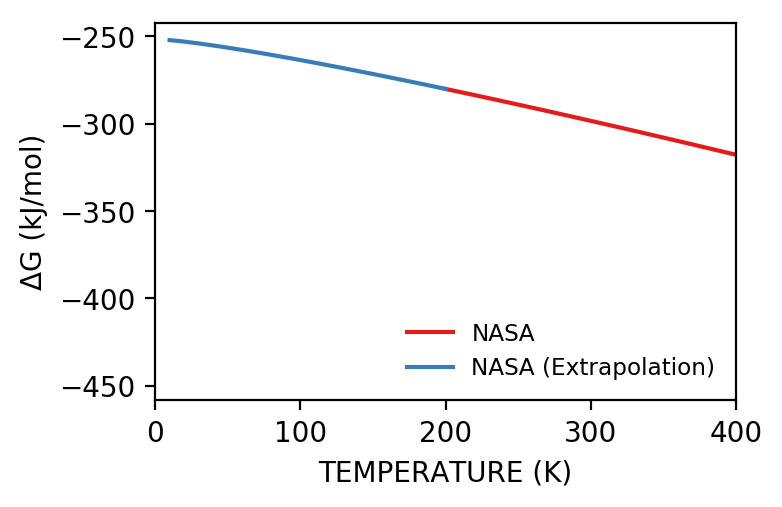
\includegraphics[width=0.70\textwidth]{zi-images/00-General-Graphics/2021-figure-H2-pMuTT.png}
    \caption{The gas phase free energy of \ce{H2} as a function of temperature. The reference state it defined as 10 K. The red line shows the NASA Polynomial within defined range, and the blue line shows the extrapolation.}
    \label{fig:h2-pmutt-expression}
\end{figure}

\begin{figure}[H]
    \centering
    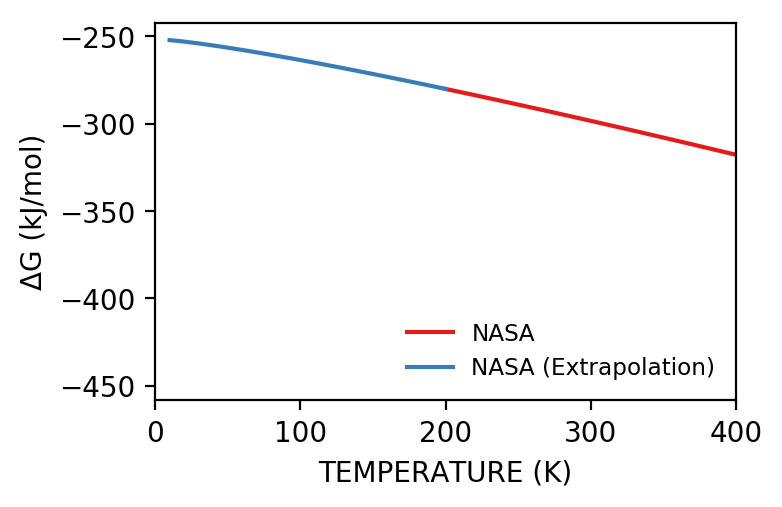
\includegraphics[width=0.70\textwidth]{zi-images/00-General-Graphics/2021-figure-H2O-pMuTT.png}
    \caption{The gas phase free energy of \ce{H2O} as a function of temperature. The reference state it defined as 10 K. The red line shows the NASA Polynomial within defined range, and the blue line shows the extrapolation.}    \label{fig:h2o-pmutt-expression}
\end{figure}

%TODO do I need a statement here about the bulk model and where the bulk models ended up coming from?

\subsection{Spin Contamination}
The library was optimized at different \ce{Ni} spin states; the considered spin states for \ce{Ni(II)} were singlet (no unpaired electrons) and triplet (two unpaired electrons). With the cluster initially containing four \ce{Ni(II)} species, the intermediate combinations were calculated (one singlet and three triplet, two singlet and two triplet, etc.). Structures that exhibited spin contamination were removed from the analysis. Comparisons between the ideal and single determinant $S^{**}2$ values were inspected. If the single determinant value deviated by more than 10\% of the ideal determinant the structure was removed from analysis. 
\begin{center}
\begin{table}[H]
\centering
  \setlength\tabcolsep{8pt}
  \caption{Example of Spin Contamination Analysis for \ce{Ni4(OH)6 \cdot 2H} Structure.}
  \label{tbl:spin_contamination}
  \begin{tabular}{lcccc}
    \hline
        \ce{Ni(II)} Spin Configuration  & \thead{ Electronic \\ Energy (hartree)} &  Ideal $S^{**}2$ &   Single $S^{**}2$ & Contamination? \\
        \hline
        a) Four singlet (RKS\textsuperscript{a}) & -4778.84071 & N\/a & N\/a & No \\
        b) Four singlet (UKS)                    & -4778.87973 & 0.000  & 2.386  & Yes \\
        c) Three singlet, one triplet            & -4778.88313 & 2.000  & 3.978  & Yes \\
        d) Two singlet, two triplet              & -4778.88042 & 6.000  & 6.457  & Yes \\
        e) One singlet, three triplet            & -4778.88209 & 12.000 & 12.014 & No \\
        f) Four triplet                          & -4778.84120 & 20.000 & 20.013 & No \\
        \hline
    \end{tabular} \\
    \textsuperscript{a} Restricted Kohn-Sham \\
\end{table}    
\end{center}
From Table \ref{tbl:spin_contamination}, the lowest energy structure is  c) three singlet, one triplet; however, the structure is removed from the analysis because the ideal $S^{**}2$ and single $S^{**}2$ deviate. Therefore, the lowest energy structure for this particular configuration is the e) one singlet, three triplet. We checked the spin state for all structures.

\newpage
\subsection{Sample Input File}
Below is a sample CP2K input file. If the singlet spin state was desired for all \ce{Ni(II)} atoms, UKS F and MULTIPLICITY 1 were used. Otherwise, UKS T was used with the appropriate MULTIPLICITY specified.
\begin{center}
    \lstset{numbers=left, basicstyle=\ttfamily, numbersep=-45pt}
    \begin{lstlisting}[language=bash]
        &GLOBAL
           PRINT_LEVEL  MEDIUM
           PROJECT_NAME info-ni4oh6-4h2o-config2-MULTI9
           RUN_TYPE  GEO_OPT
           WALLTIME 71:47:00
         &END GLOBAL
         &MOTION
           &GEO_OPT
             TYPE  MINIMIZATION
             OPTIMIZER  BFGS
             MAX_ITER  2000
             MAX_DR     5.0000000000000001E-04
             MAX_FORCE     5.0000000000000002E-05
             RMS_DR     5.0000000000000001E-04
             RMS_FORCE     5.0000000000000002E-05
             STEP_START_VAL  603
             &BFGS
               TRUST_RADIUS     2.5000000000000006E-01
             &END BFGS
           &END GEO_OPT
         &END MOTION
         &FORCE_EVAL
           METHOD  QS
           STRESS_TENSOR  ANALYTICAL
           &DFT
             BASIS_SET_FILE_NAME BASIS_file
             POTENTIAL_FILE_NAME POTENTIALS_file
             UKS  T
             MULTIPLICITY  9
             CHARGE  0
             &SCF
               MAX_SCF  1000
               EPS_SCF     9.9999999999999995E-07
               SCF_GUESS  ATOMIC
               &OT  T
                 MINIMIZER  CG
                 PRECONDITIONER  FULL_ALL
                 ENERGY_GAP     1.0000000000000000E-03
               &END OT
               &OUTER_SCF  T
                 EPS_SCF     9.9999999999999995E-07
                 MAX_SCF  50
               &END OUTER_SCF
             &END SCF
             &QS
               EPS_DEFAULT     1.0000000000000000E-10
               METHOD  GPW
             &END QS
             &MGRID
               NGRIDS  5
               CUTOFF     3.6000000000000000E+02
               REL_CUTOFF     8.0000000000000000E+01
             &END MGRID
             &XC
               DENSITY_CUTOFF     1.0000000000000000E-10
               GRADIENT_CUTOFF     1.0000000000000000E-10
               TAU_CUTOFF     1.0000000000000000E-10
               &XC_FUNCTIONAL  NO_SHORTCUT
                 &PBE  T
                 &END PBE
               &END XC_FUNCTIONAL
               &VDW_POTENTIAL
                 POTENTIAL_TYPE  PAIR_POTENTIAL
                 &PAIR_POTENTIAL
                   TYPE  DFTD3(BJ)
                   PARAMETER_FILE_NAME dftd3.dat
                   REFERENCE_FUNCTIONAL PBE
                   CALCULATE_C9_TERM  F
                 &END PAIR_POTENTIAL
               &END VDW_POTENTIAL
             &END XC
           &END DFT
           &SUBSYS
             &CELL
               A     4.061108E+01   0.00000E+00    0.00000E+00
               B     2.03054E+01    3.51702E+01    0.00000E+00
               C     0.00000E+00    0.00000E+00    1.59897E+01
               MULTIPLE_UNIT_CELL  1 1 1
               SYMMETRY  MONOCLINIC_GAMMA_AB
             &END CELL
             &KIND C
               BASIS_SET DZVP-MOLOPT-SR-GTH-q4
               POTENTIAL GTH-PBE-q4
             &END KIND
             &KIND H
               BASIS_SET DZVP-MOLOPT-SR-GTH-q1
               POTENTIAL GTH-PBE-q1
             &END KIND
             &KIND Ni
               BASIS_SET DZVP-MOLOPT-SR-GTH-q18
               POTENTIAL GTH-PBE-q18
             &END KIND
             &KIND O
               BASIS_SET DZVP-MOLOPT-SR-GTH-q6
               POTENTIAL GTH-PBE-q6
             &END KIND
             &KIND Zr
               BASIS_SET DZVP-MOLOPT-SR-GTH-q12
               POTENTIAL GTH-PBE-q12
             &END KIND
             &TOPOLOGY
               COORD_FILE_NAME ./sNi4OH6-4H2O-config2.xyz
               COORD_FILE_FORMAT  XYZ
               NUMBER_OF_ATOMS  584
               CONN_FILE_FORMAT  OFF
               MULTIPLE_UNIT_CELL  1 1 1
             &END TOPOLOGY
           &END SUBSYS
           &PRINT
             &FORCES  ON
             &END FORCES
           &END PRINT
         &END FORCE_EVAL
    \end{lstlisting}
\end{center}

\newpage
\subsection{Sample Input File for bulk Ni}
Below is a sample CP2K input file. If the singlet spin state was desired for all \ce{Ni(II)} atoms, UKS F and MULTIPLICITY 1 were used. Otherwise, UKS T was used with the appropriate MULTIPLICITY specified.
\begin{center}
    \lstset{numbers=left, basicstyle=\ttfamily, numbersep=-45pt}
    \begin{lstlisting}[language=bash]
        &GLOBAL
          PRINT_LEVEL low
          PROJECT_NAME Ni-MULTI9
          RUN_TYPE cell_opt
        &END GLOBAL
        &MOTION
          &CELL_OPT
            EXTERNAL_PRESSURE [bar] 1.0
            MAX_DR 0.001
            MAX_FORCE 0.0001
            MAX_ITER 400
            OPTIMIZER BFGS
            PRESSURE_TOLERANCE [bar] 10.0
            RMS_DR 0.0003
            RMS_FORCE 0.00003
            TYPE direct_cell_opt
            &BFGS
              TRUST_RADIUS 0.1
              USE_MODEL_HESSIAN off
              USE_RAT_FUN_OPT on
            &END BFGS
          &END CELL_OPT
        &END MOTION
        &FORCE_EVAL
          METHOD QS
          STRESS_TENSOR analytical
          &DFT
            BASIS_SET_FILE_NAME ./BASIS_file
            POTENTIAL_FILE_NAME ./POTENTIALS_file
            &KPOINTS
              SCHEME MONKHORST-PACK 6 6 6
              FULL_GRID yes
              SYMMETRY yes
              VERBOSE yes
              PARALLEL_GROUP_SIZE -1
            &END KPOINTS
            &MGRID
              NGRIDS 5
              CUTOFF 400.0
              REL_CUTOFF 60.0
            &END MGRID
            &QS
              EPS_DEFAULT 1.0E-12
              EXTRAPOLATION use_prev_p
            &END QS
            &SCF
              ADDED_MOS 60
              EPS_SCF 1.0E-8
              MAX_SCF 300
              SCF_GUESS restart
              &DIAGONALIZATION yes
                ALGORITHM STANDARD
              &END DIAGONALIZATION
              &MIXING yes
                ALPHA 0.4
                BETA 1.0
                METHOD broyden_mixing
                NBROYDEN 8
              &END MIXING
              &SMEAR on
                METHOD FERMI_DIRAC
                ELECTRONIC_TEMPERATURE [K] 2000.0
              &END SMEAR
            &END SCF
            &XC
              &XC_FUNCTIONAL PBE
              &END XC_FUNCTIONAL
              &VDW_POTENTIAL
                POTENTIAL_TYPE pair_potential
                &PAIR_POTENTIAL
                  TYPE DFTD3(BJ)
                  PARAMETER_FILE_NAME dftd3.dat
                  REFERENCE_FUNCTIONAL PBE
                &END PAIR_POTENTIAL
              &END VDW_POTENTIAL
            &END XC
          &END DFT
          &SUBSYS
            &CELL
              ABC 3.50 3.50 3.50
              MULTIPLE_UNIT_CELL 2 2 2
            &END CELL
            &COORD
              SCALED
              Ni    0    0    0
              Ni    0  1/2  1/2
              Ni  1/2    0  1/2
              Ni  1/2  1/2    0
            &END COORD
            &KIND Ni
              BASIS_SET DZVP-MOLOPT-SR-GTH-q18
              POTENTIAL GTH-PBE-q18
            &END KIND
            &TOPOLOGY
              MULTIPLE_UNIT_CELL 2 2 2
            &END TOPOLOGY
          &END SUBSYS
        &END FORCE_EVAL
    \end{lstlisting}
\end{center}

    \newpage
    
    
\section{Influence of \ce{H2O} partial pressure on the thermodynamic stability.}
\begin{figure}[H]
    \centering
    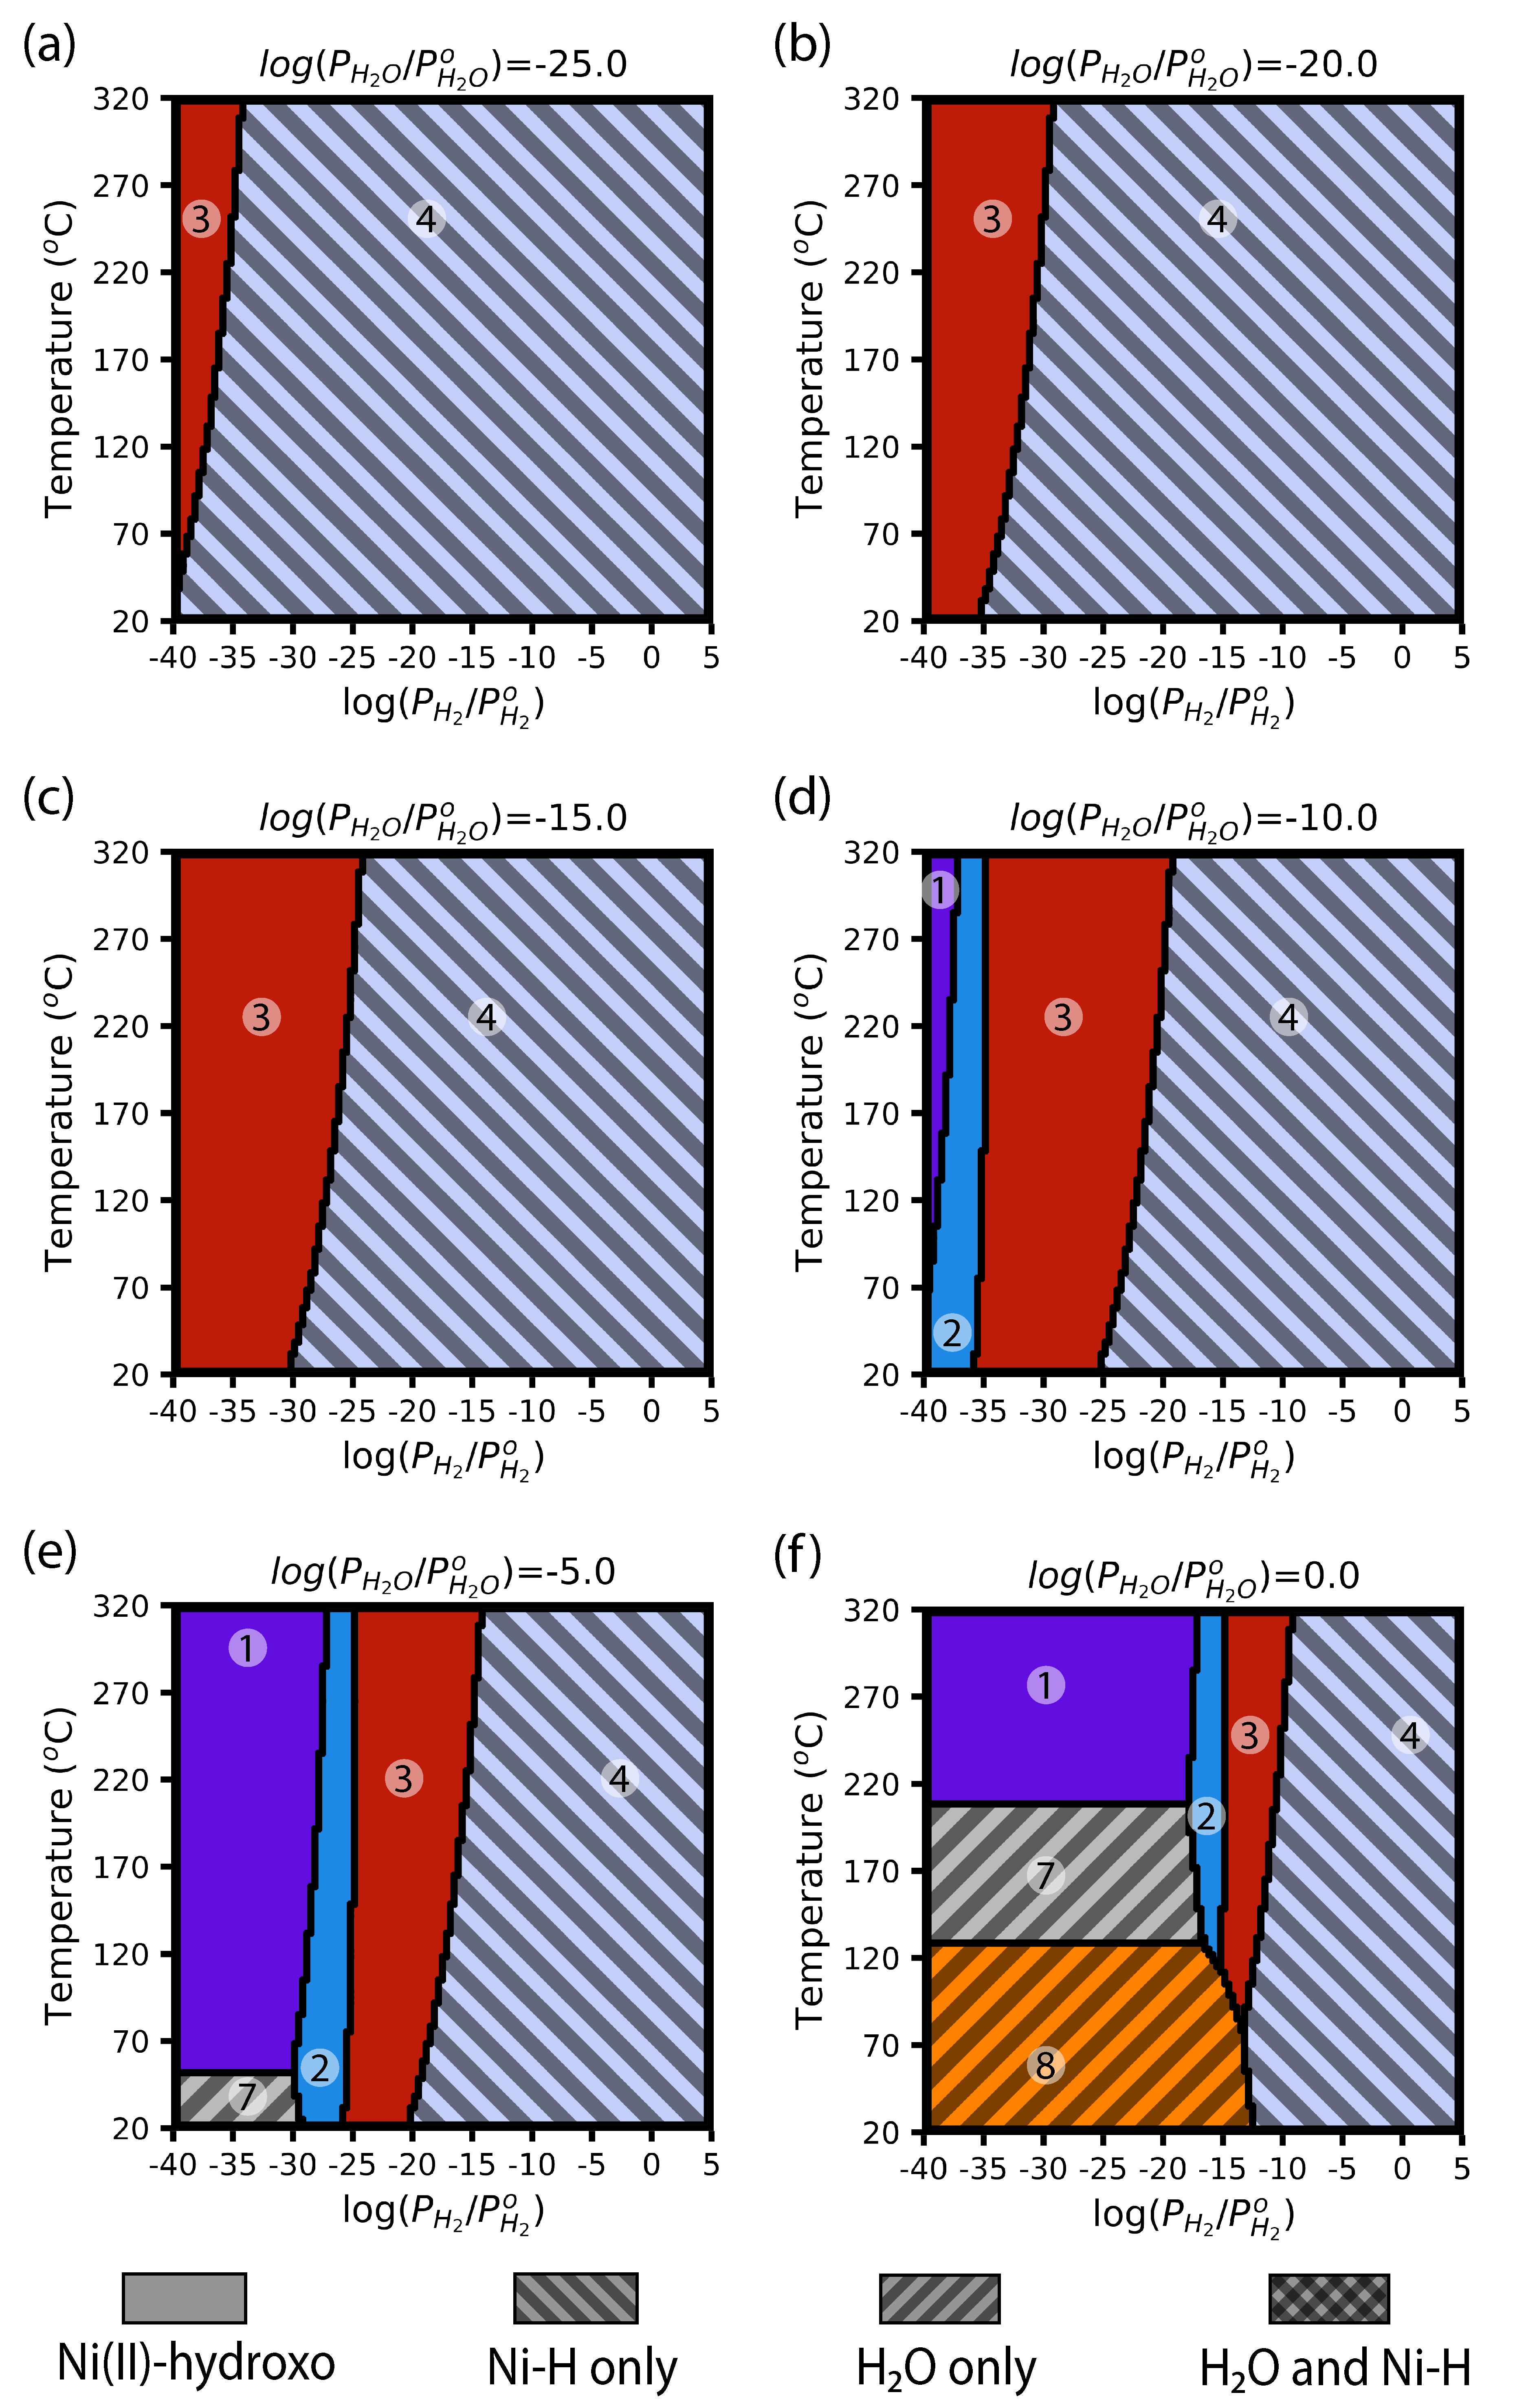
\includegraphics[width=0.60\linewidth]{zi-images/04-SI-images/2021-05-04-Trans-Ni.png}
    \caption{
    The thermodynamic stability of the cluster is plotted as a function of \ce{H2O} partial pressure from $10^{-25}$ to $10^{0.0}$ bar for a variable \ce{Ni} composition. The structures present on the phase diagram include:
        1-\ce{Ni4(OH)6} (purple),               % purple 
        2-\ce{Ni4(OH)4} (blue),                 % blue
        3-\ce{Ni3(OH)2} (red),                  % red 
        4-\ce{Ni2(H)2} (lilac),                 % lilac 
        5-\ce{Ni4(H)2} (mint),                  % mint
        7-\ce{Ni4(OH)6.H2O} (gray), and         % gray
        8-\ce{Ni4(OH)6.4H2O} (orange).          % orange
    With increasing \ce{H2O} partial pressure, the \ce{Ni} atoms remain highly coordinated because \ce{OH}-ligands and any coordinated \ce{H2O} remain on the cluster.  
    }
    \label{fig:SI-phase-Ni-trans}
\end{figure}

\begin{figure}[H]
    \centering
    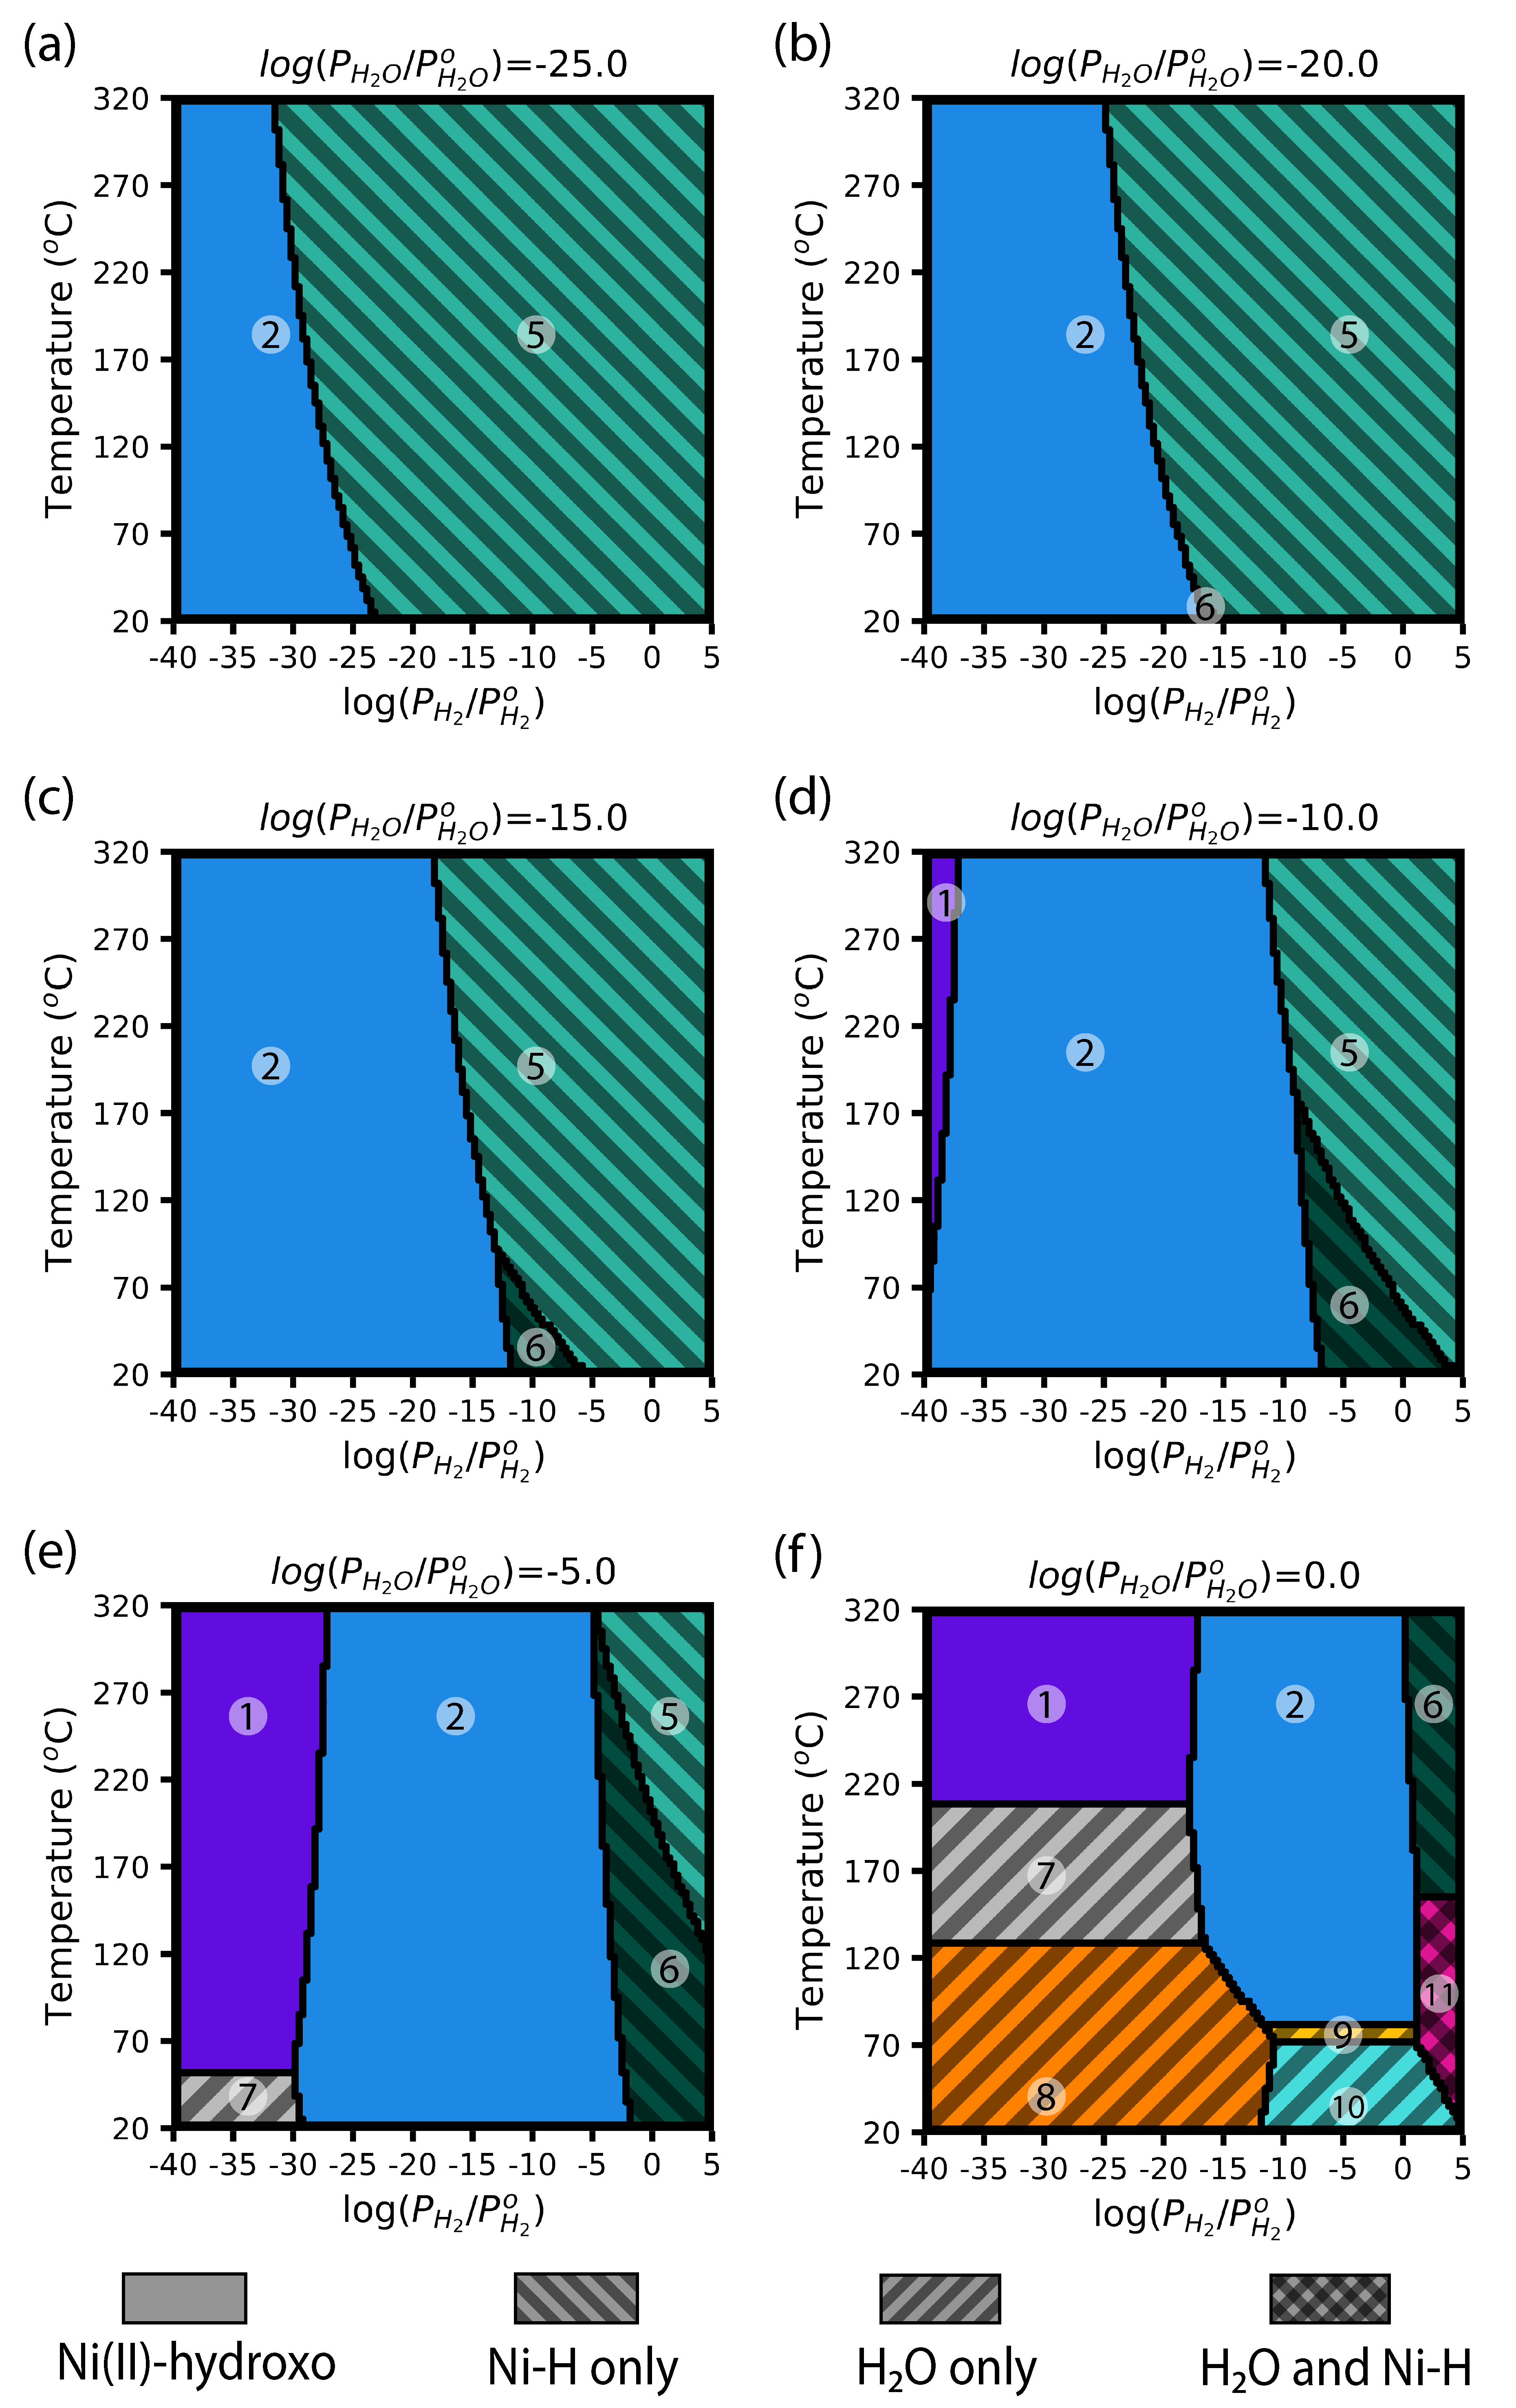
\includegraphics[width=0.60\linewidth]{zi-images/04-SI-images/2021-05-04-Fixed-Ni.png}
    \caption{
    The thermodynamic stability of the cluster is plotted as a function of \ce{H2O} partial pressure from $10^{-25}$ to $10^{0.0}$ bar for a fixed \ce{Ni} composition. The structures present on the phase diagram include:
        1-\ce{Ni4(OH)6} (purple),               % purple 
        2-\ce{Ni4(OH)4} (blue),                 % blue
        5-\ce{Ni4(H)2} (mint),                  % mint
        6-\ce{Ni4(OH)2(H)2} (green),            % green
        7-\ce{Ni4(OH)6.H2O} (gray),             % gray
        8-\ce{Ni4(OH)6.4H2O} (orange),          % orange
        9-\ce{Ni4(OH)4.H2O} (yellow),           % yellow
        10-\ce{Ni4(OH)5(H).4H2O} (teal), and    % teal
        11-\ce{Ni4(OH)2(H)2.H2O} (pink).        % pink
    With increasing \ce{H2O} partial pressure, the \ce{Ni} atoms remain highly coordinated because \ce{OH}-ligands and any coordinated \ce{H2O} remain on the cluster.  
    }
    \label{fig:SI-phase-Ni-fixed}
\end{figure}

We highlight the importance of \ce{H2O} partial pressure on the thermodynamic stability of the \ce{Ni4} cluster. Both Figure \ref{fig:SI-phase-Ni-trans} and Figure \ref{fig:SI-phase-Ni-fixed} show the evolution of the phase diagram as a function of \ce{H2O} partial pressure. Experimentally, the \ce{H2O} partial pressure is assumed to be small. However, we have no method for quantifying how small the partial pressure is. Therefore, we select an \ce{H2O} partial pressure of $10^{-10}$ bar for both the variable and fixed \ce{Ni} phase diagrams presented within the manuscript. Ultra-high vacuum conditions range from $10^{-10}$ to $10^{-15}$ bar, so our selected \ce{H2O} partial pressure is within that range. \citeauthor{PlateroPrats2017} observed a \ce{Ni} coordination number of approximately 5,\cite{PlateroPrats2017} which we only observe at larger \ce{H2O} partial pressure.

\newpage
\section{Structure diagram for all phase diagram structures.}
\begin{figure}[H]
    \centering
    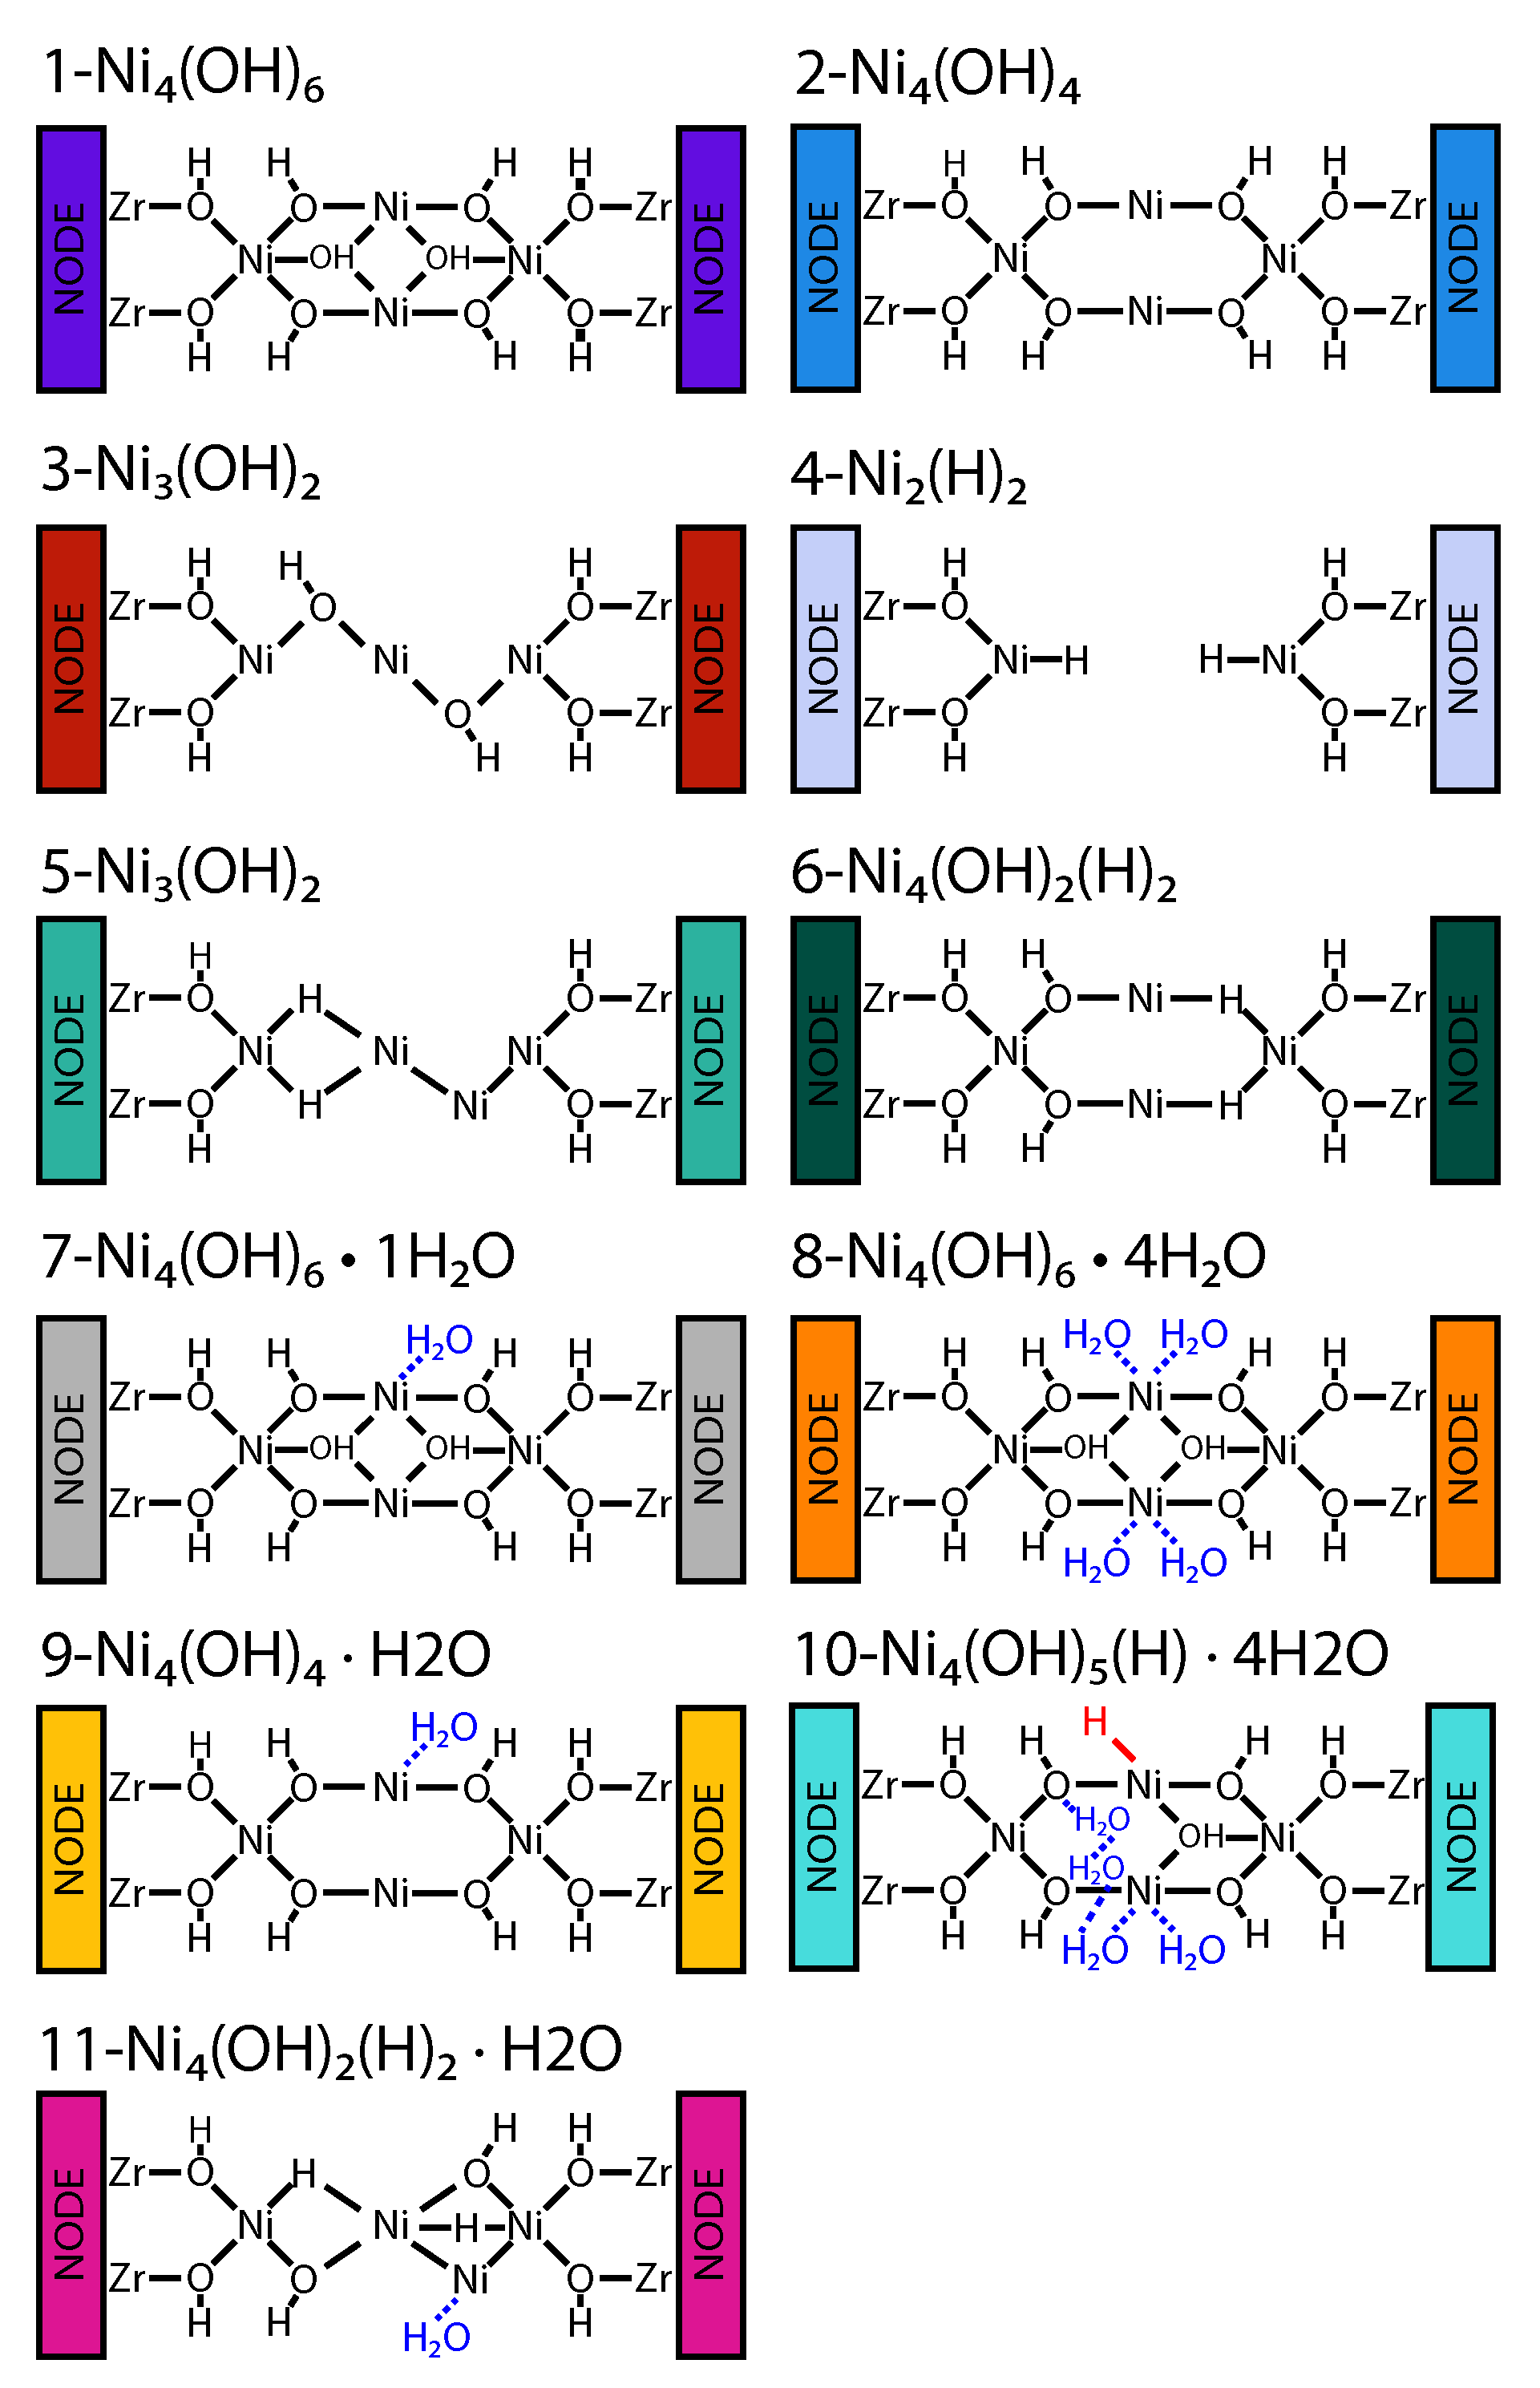
\includegraphics{zi-images/04-SI-images/2021-05-11-updated-manuscript-structure-SI-ALL.png}
    \caption{
    All the structures located on Figures \ref{fig:SI-phase-Ni-trans} and \ref{fig:SI-phase-Ni-fixed} are shown. The same naming convention and color scheme is used as the phase diagram figure. The structures shown are: 
        1-\ce{Ni4(OH)6} (purple),               % purple 
        2-\ce{Ni4(OH)4} (blue),                 % blue
        5-\ce{Ni4(H)2} (mint),                  % mint
        6-\ce{Ni4(OH)2(H)2} (green),            % green
        7-\ce{Ni4(OH)6.H2O} (gray),             % gray
        8-\ce{Ni4(OH)6.4H2O} (orange),          % orange
        9-\ce{Ni4(OH)4.H2O} (yellow),           % yellow
        10-\ce{Ni4(OH)5(H).4H2O} (teal), and    % teal
        11-\ce{Ni4(OH)2(H)2.H2O} (pink).        % pink
    }
    \label{fig:SI-structure-diagram}
\end{figure}

\section{dPDF diagram for all phase diagram structures.}
\begin{figure}[H]
    \centering
    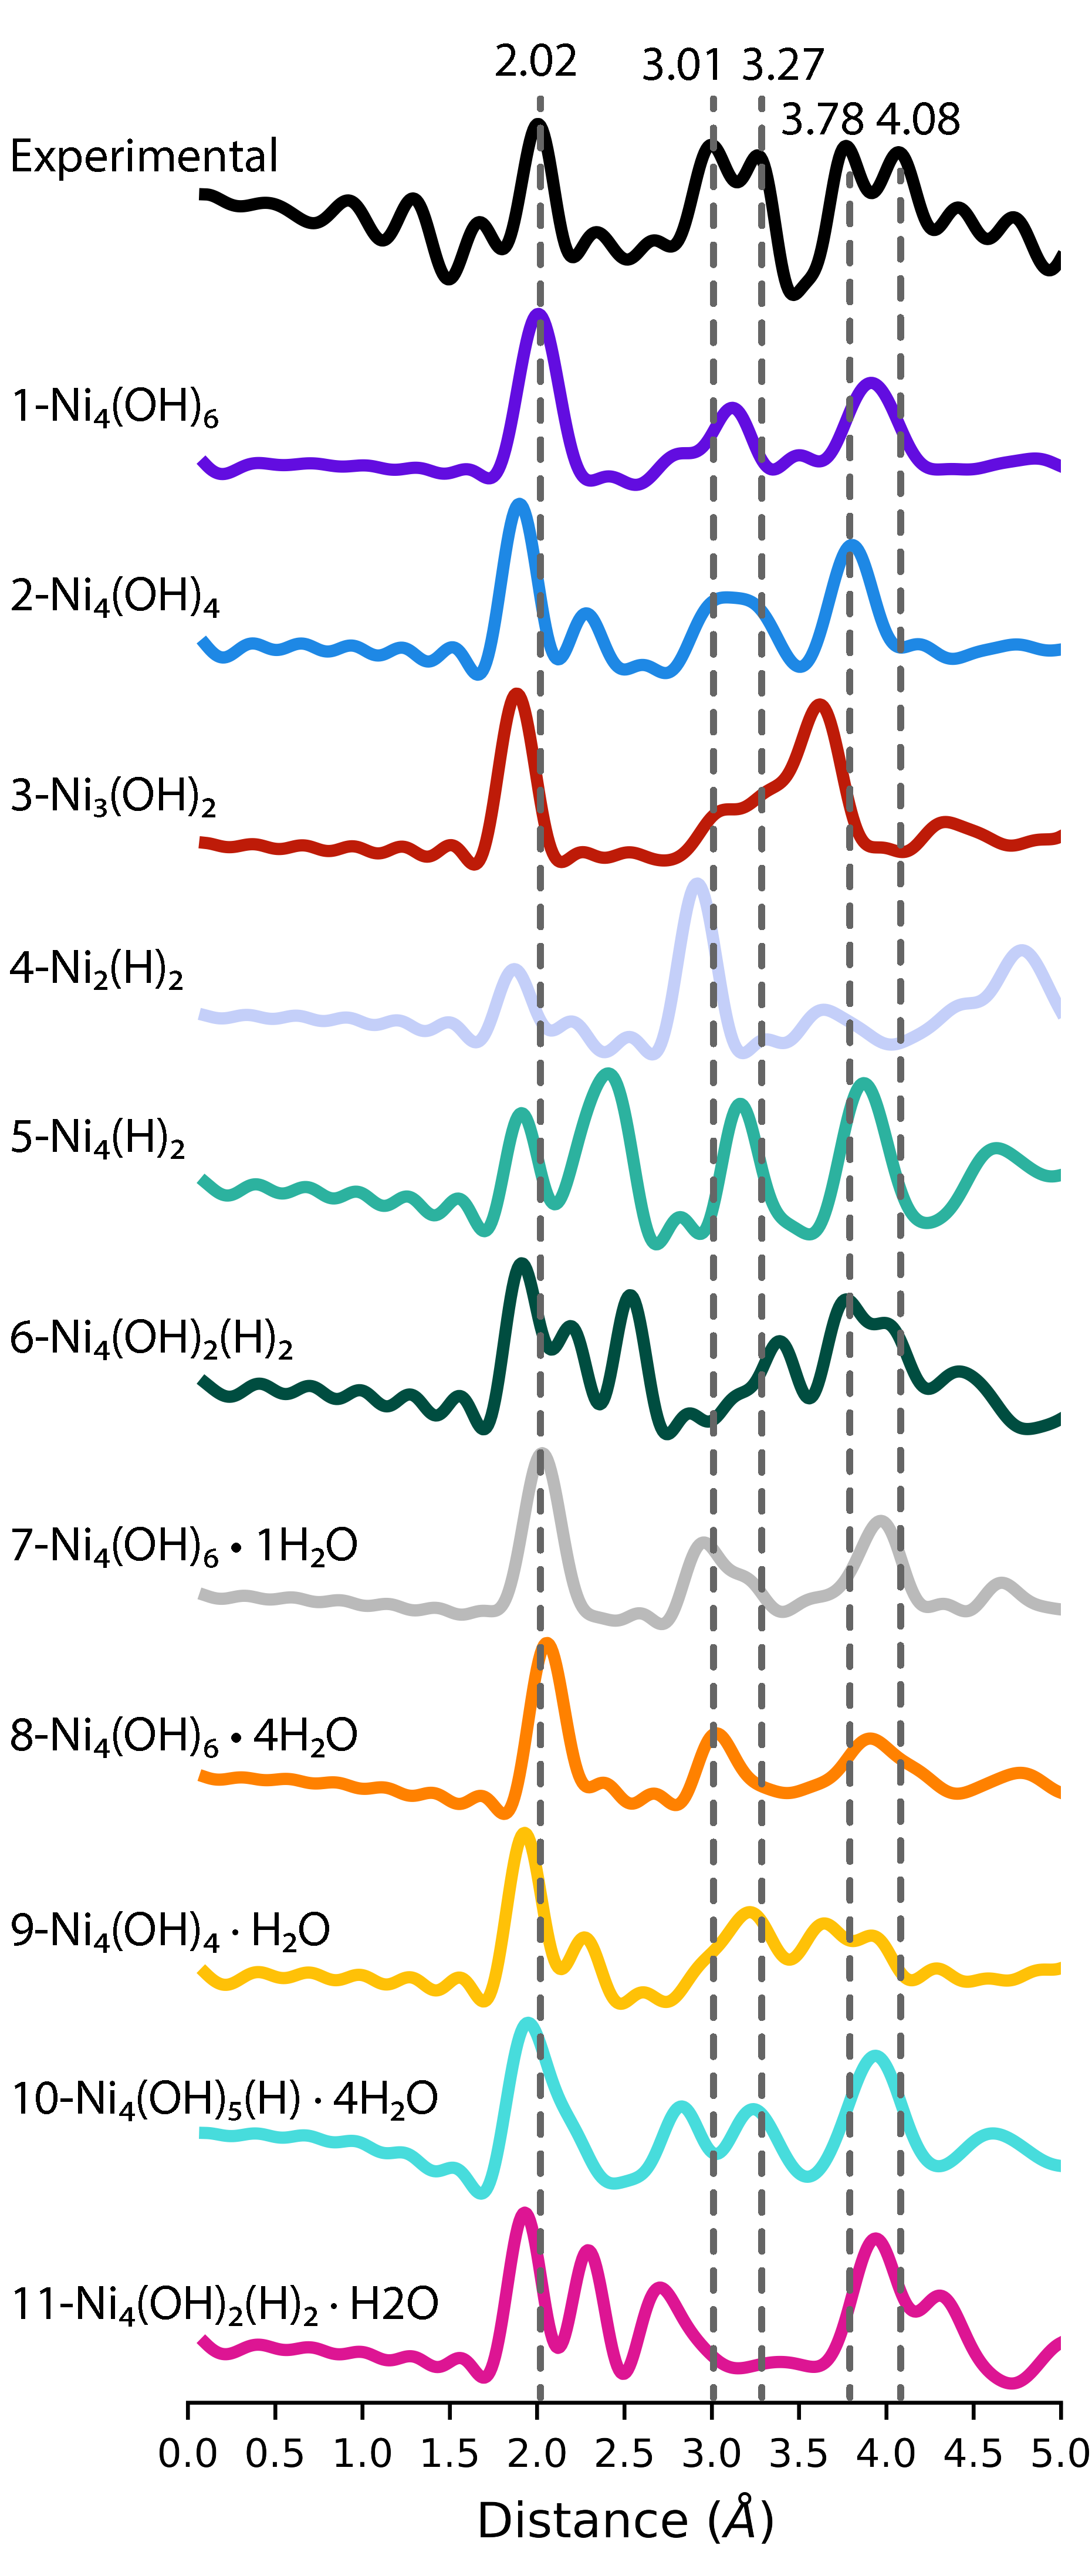
\includegraphics{zi-images/04-SI-images/2021-05-11-Ni-single-dPDF-ALL-SI-ALL.png}
    \caption{
    The dPDFs for the structure located on Figure \ref{fig:SI-phase-Ni-trans} (variable \ce{Ni} content) and \ref{fig:SI-phase-Ni-fixed} (fixed \ce{Ni} content). The same naming convention and color is used as illustrated on previous figures. The dPDFs for the following structures are shown:
        1-\ce{Ni4(OH)6} (purple),               % purple 
        2-\ce{Ni4(OH)4} (blue),                 % blue
        5-\ce{Ni4(H)2} (mint),                  % mint
        6-\ce{Ni4(OH)2(H)2} (green),            % green
        7-\ce{Ni4(OH)6.H2O} (gray),             % gray
        8-\ce{Ni4(OH)6.4H2O} (orange),          % orange
        9-\ce{Ni4(OH)4.H2O} (yellow),           % yellow
        10-\ce{Ni4(OH)5(H).4H2O} (teal), and    % teal
        11-\ce{Ni4(OH)2(H)2.H2O} (pink).        % pink
    }
    \label{fig:SI-structure-diagram}
\end{figure}

\newpage
\section{Structure diagram for structure containing a NiH species}
\begin{figure}[H]
    \centering
    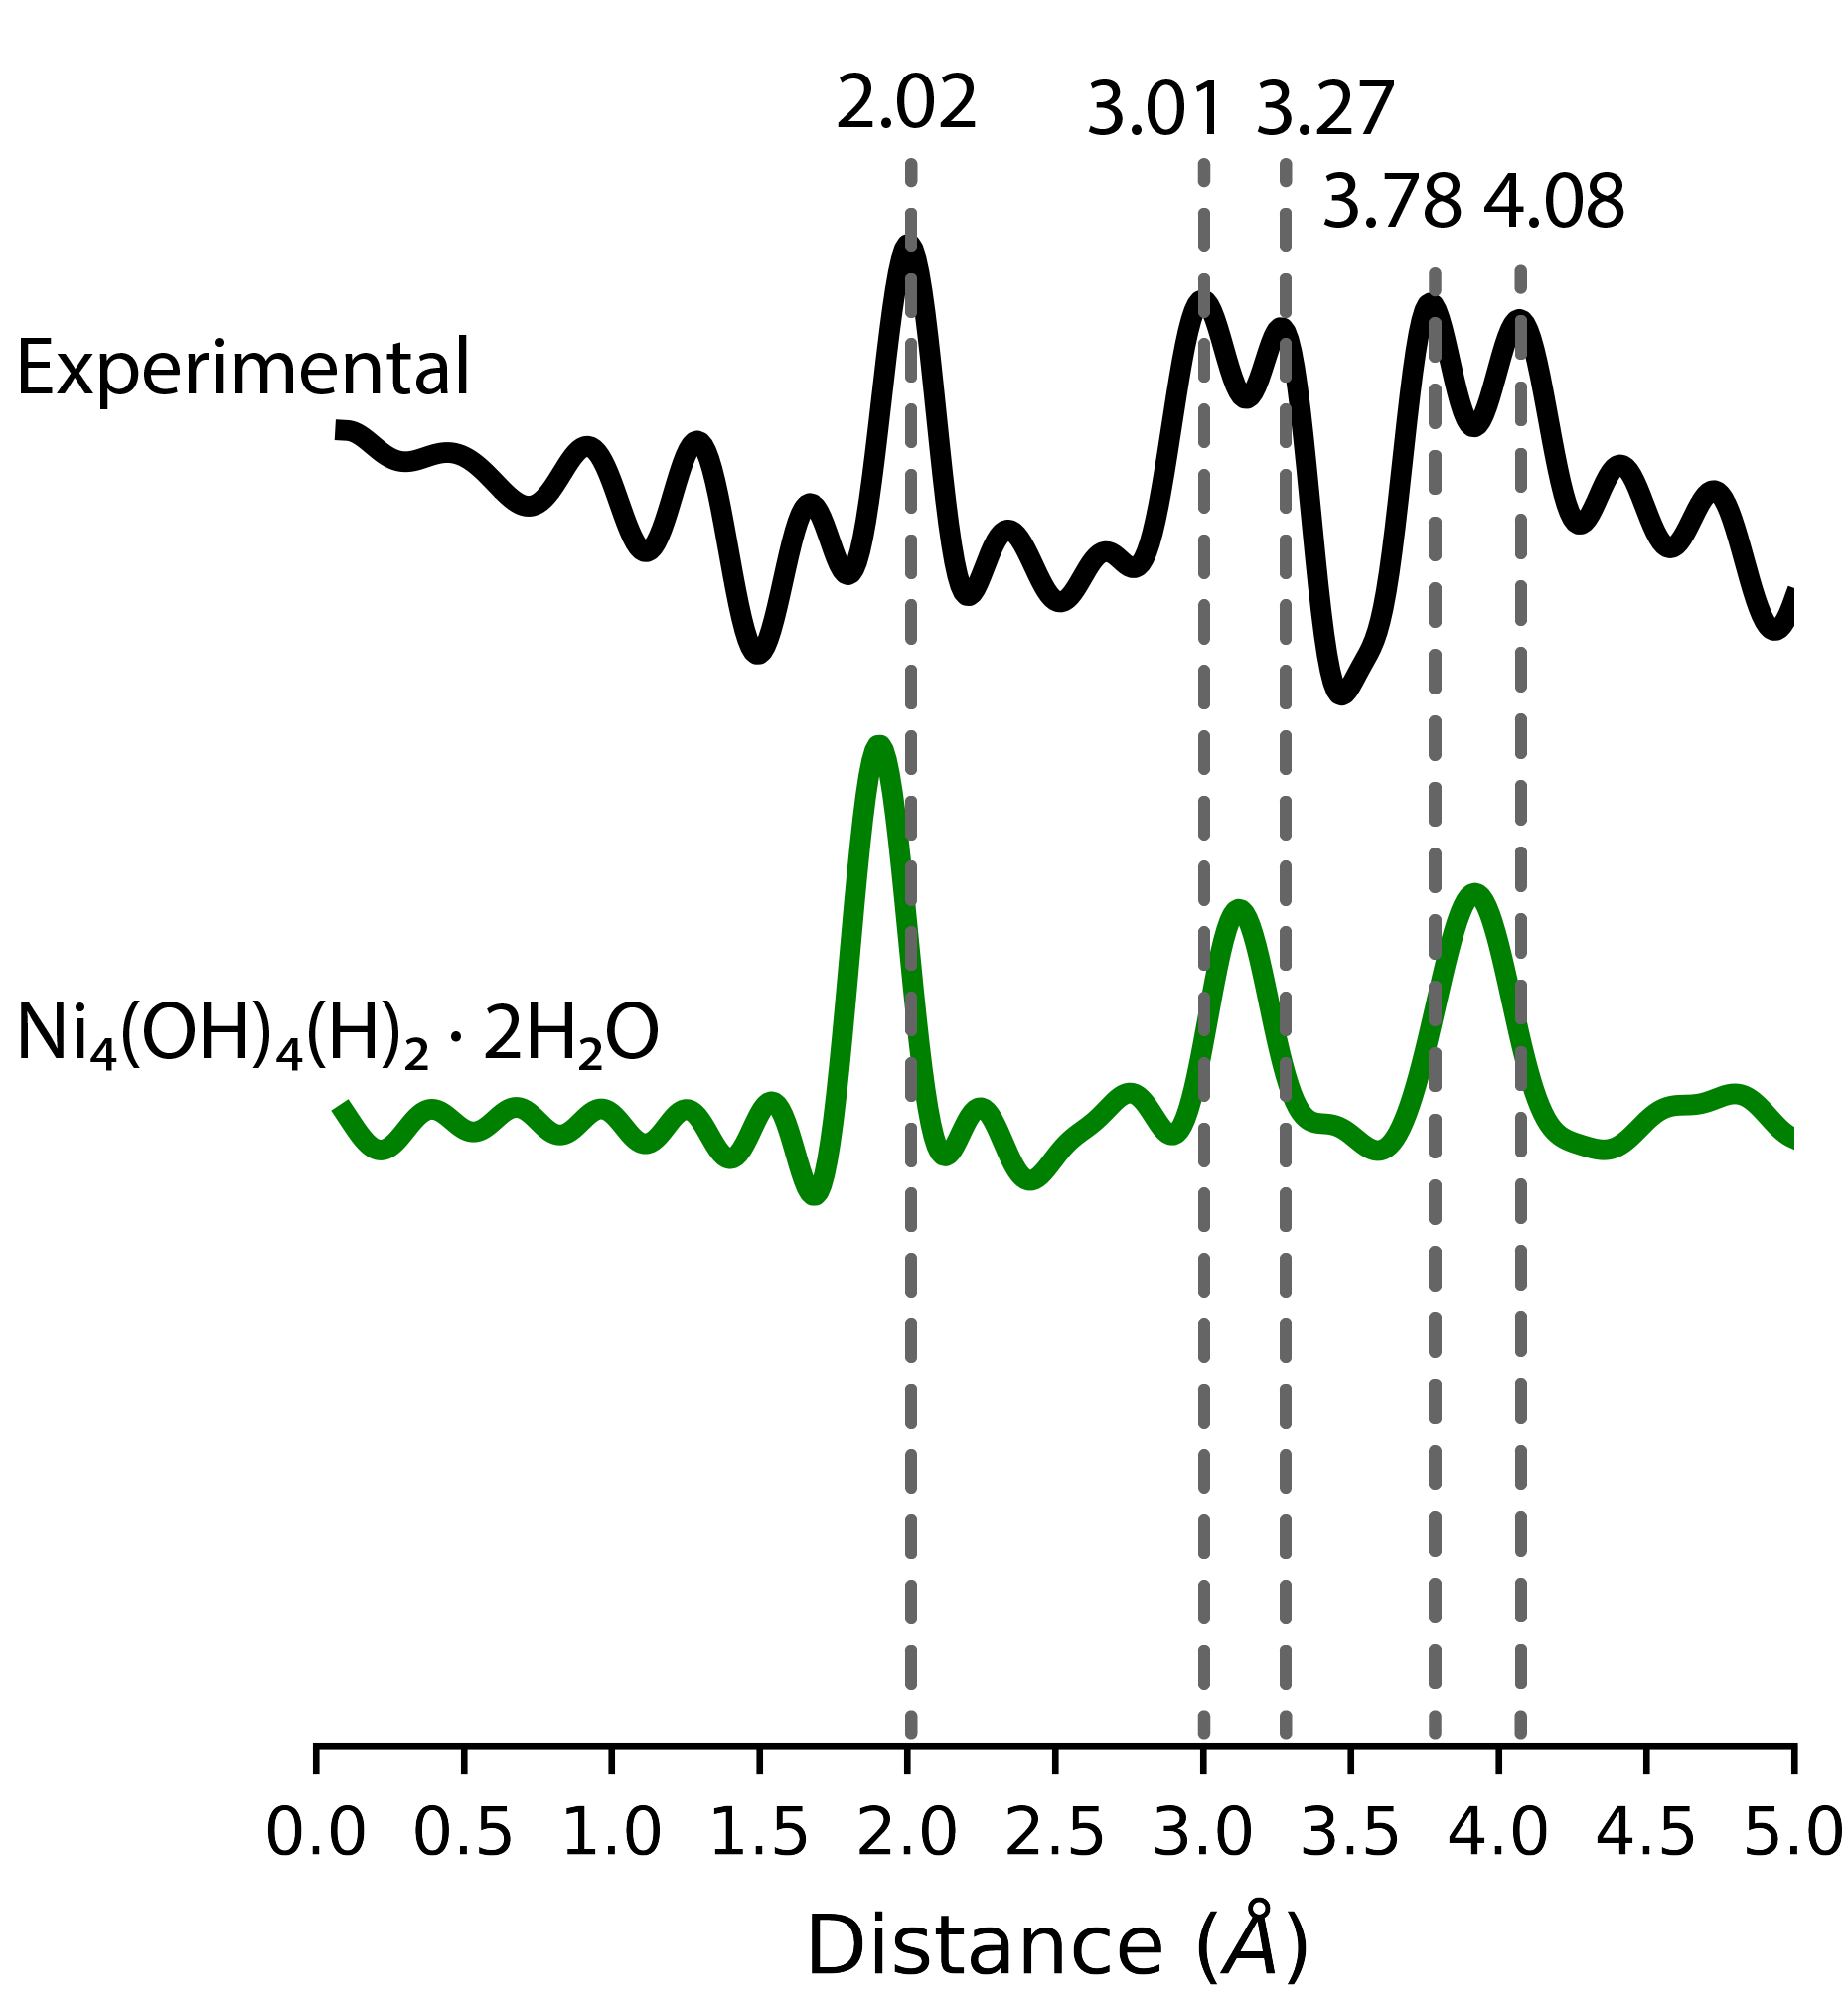
\includegraphics{zi-images/04-SI-images/2021-05-10-Ni-single-dPDF-Ni-H.png}
    \caption{
    The dPDFs and structure diagrams for structures that feature a traditional \ce{Ni-H} species. The * denotes structures that are not thermodynamic minimum on during any of the \textit{ab initio} thermodynamic analysis. \hl{Statement about the structures here.. need to explain some of the key features from the dPDFs and what that means in the context of the story.}
    }
    \label{fig:SI-structure-diagram}
\end{figure}


\newpage
\section{References}

%The class makes various changes to the way that references are
%handled.  The class loads \textsf{natbib}, and also the
%appropriate bibliography style.  References can be made using
%the normal method; the citation should be placed before any
%punctuation, as the class will move it if using a superscript
%citation style
%\cite{Mena2000,Abernethy2003,Friedman-Hill2003,EuropeanCommission2008}.
%The use of \textsf{natbib} allows the use of the various citation
%commands of that package: \citeauthor{Abernethy2003} have shown
%something, in \citeyear{Cotton1999}, or as given by
%Ref.~\citenum{Mena2000}.  Long lists of authors will be
%automatically truncated in most article formats, but not in
%supplementary information or reviews \cite{Pople2003}. If you
%encounter problems with the citation macros, please check that
%your copy of \textsf{natbib} is up to date. The demonstration
%database file \texttt{achemso-demo.bib} shows how to complete
%entries correctly. Notice that ``\latin{et al.}'' is auto-formatted
%using the \texttt{\textbackslash latin} command.

%Multiple citations to be combined into a list can be %given as
%a single citation.  This uses the \textsf{mciteplus} %package
%\cite{Johnson1972,*Arduengo1992,*Eisenstein2005,*Arduengo%1994}.
%Citations other than the first of the list should be %indicated
%with a star. If the \textsf{mciteplus} package is not %installed,
%the standard bibliography tools will still work but %starred
%references will be ignored. Individual references can be %referred
%to using \texttt{\textbackslash mciteSubRef}:
%``ref.~\mciteSubRef{Eisenstein2005}''.

%The class also handles notes to be added to the bibliography.  These
%should be given in place in the document \bibnote{This is a note.
%The text will be moved the the references section.  The title of the
%section will change to ``Notes and References''.}.  As with
%citations, the text should be placed before punctuation.  A note is
%also generated if a citation has an optional note.  This assumes that
%the whole work has already been cited: odd numbering will result if
%this is not the case \cite[p.~1]{Cotton1999}.

%%%%%%%%%%%%%%%%%%%%%%%%%%%%%%%%%%%%%%%%%%%%%%%%%%%%%%%%%%%%%%%%%%%%%
%% The "Acknowledgement" section can be given in all manuscript
%% classes.  This should be given within the "acknowledgement"
%% environment, which will make the correct section or running title.
%%%%%%%%%%%%%%%%%%%%%%%%%%%%%%%%%%%%%%%%%%%%%%%%%%%%%%%%%%%%%%%%%%%%%
%\begin{acknowledgement}
%
%\hl{authors would like to thank \ldots''.
%
%The author thanks Mats Dahlgren for version one of \textsf{achemso},
%and Donald Arseneau for the code taken from \textsf{cite} to move
%citations after punctuation. Many users have provided feedback on the
%class, which is reflected in all of the different demonstrations
%shown in this document.}
%
%\end{acknowledgement}

%%%%%%%%%%%%%%%%%%%%%%%%%%%%%%%%%%%%%%%%%%%%%%%%%%%%%%%%%%%%%%%%%%%%%
%% The same is true for Supporting Information, which should use the
%% suppinfo environment.
%%%%%%%%%%%%%%%%%%%%%%%%%%%%%%%%%%%%%%%%%%%%%%%%%%%%%%%%%%%%%%%%%%%%%
%\begin{suppinfo}
%
%\hl{This will usually read something like: ``Experimental procedures and
%characterization data for all new compounds. The class will
%automatically add a sentence pointing to the information on-line:}
%
%\end{suppinfo}

%%%%%%%%%%%%%%%%%%%%%%%%%%%%%%%%%%%%%%%%%%%%%%%%%%%%%%%%%%%%%%%%%%%%%
%% The appropriate \bibliography command should be placed here.
%% Notice that the class file automatically sets \bibliographystyle
%% and also names the section correctly.
%%%%%%%%%%%%%%%%%%%%%%%%%%%%%%%%%%%%%%%%%%%%%%%%%%%%%%%%%%%%%%%%%%%%%
\bibliography{achemso-demo}

\end{document}